\documentclass{report}

%--- Packages ---
\usepackage{graphicx}                % Required for inserting images
	\graphicspath{ {./pictures/} }
\usepackage{svg} %for SVGs

\usepackage{wrapfig}
\usepackage{fancyhdr}      % Paket für Kopf- und Fusszeilen
\usepackage{lastpage}
\usepackage[hidelinks]{hyperref}     % Paket für Hyperlinks
\hypersetup{
	colorlinks=true,
	citecolor=olive,
	linkcolor=blue,
	filecolor=magenta,      
	urlcolor=cyan,
	pdftitle={Overleaf Example},
	pdfpagemode=FullScreen,
}
\renewcommand{\footnoterule}{\vfill\kern -3pt \hrule width 0.4\columnwidth \kern 2.6pt}
\usepackage[table]{xcolor}                  % Paket für Farbliche Highlights
\usepackage{float}                   % Im Dokumenten-Präambel hinzufügen
\usepackage{pdflscape} 
\usepackage{amsmath}
\usepackage{pgfplots}
\usepackage[utf8]{inputenc}  % Zeichencodierung für Umlaute und Sonderzeichen
\usepackage{url}             % Für die korrekte Darstellung von URLs

\usepackage{tabularx}
\usepackage{booktabs}
\usepackage{arydshln} % Gestrichelte Linien

\usepackage{caption}
\usepackage{longtable}
\usepackage{pdfpages}
\usepackage{multimedia}
\usepackage{subcaption}

%Line spacing
\usepackage{setspace}
\renewcommand{\baselinestretch}{1.5} 

\usepackage{tocloft}
\usepackage{etoolbox} % Für Änderungen an \printbibliography

%Font
\usepackage{fontspec}
\setmainfont{FiraSans}

% Bibliography
\usepackage[backend=bibtex,style=authortitle]{biblatex}
\nocite{*} 
\addbibresource{bibliography.bib}

\captionsetup{justification=centering}


% Language setting
\usepackage[german]{babel}

% Set page size and margins
% Papier Format A4
\usepackage[
	a4paper,
	top=2cm,
	bottom=2cm,
	left=2.1cm,
	right=2.1cm,
	marginparwidth=1.75cm,
	%headsep=4mm,
	%voffset=4mm,
	%tmargin=7mm,
	headheight=8mm
	]
{geometry}

%Nummerierung anpassen
\renewcommand{\thesection}{\arabic{section}}
\title{Design und Herstellung eines Beam Steering-fähigen Saiteninstruments}
\author{Nathanael Gubler}
\date{\today}

% Fußzeilen definieren
\pagestyle{fancy}  	% Aktiviert fancyhdr für Kopf- und Fußzeilen
\fancyhf{}  		% Alle vorherigen Kopf- und Fußzeilen löschen


% Logo in der Kopfzeile rechts
\fancyhead[R]{
	\includegraphics[width=6cm]{./pictures/JuventusLogo.pdf}
	%\vspace{3mm}
	} % Logo rechts
\fancyfoot[C]{\thepage}
% Kopfzeilenlinie entfernen
\renewcommand{\headrulewidth}{1pt}
\renewcommand{\footrulewidth}{2pt}

% Fußzeile: links, mitte und rechts
\fancyfoot[C]{Seite \thepage~von~\pageref{LastPage}}   	% Fußzeile in der Mitte
\fancyfoot[R]{\today}           						% Fußzeile rechts
\fancyfoot[L]{
	\begin{minipage}{6cm}
		Design und Herstellung eines \textit{Beam Steering}-fähigen Saiteninstruments
	\end{minipage}
	}      				% Fußzeile links

\begin{document}
%--- Title Page with Image
\setstretch{1.5}
\begin{titlepage}
	\setstretch{3}
	\thispagestyle{empty} % No footer on the title page
	\begin{center}
		 \vspace*{75pt} % Push content to vertical center
		
		% Title
		{ \huge \textbf{Design und Herstellung eines Beam Steering-fähigen Saiteninstruments}} 			\\ [0.5cm]
		{\Large Nathanael Gubler}\\TS TSE 2302 A\\ [1.0cm]
		\includegraphics[width=6.0cm]{./pictures/JuventusLogo.pdf} 	\\ [0.5cm]
		{\large Juventus Technikerschule HF\\Betreuer: Martin Burger} 			\\ [0.5cm]
		{\large \today} 											\\ [1.0cm]
		\vspace*{-700pt}
		% Insert the image spacing below the image
		%\begin{figure}[H]
		%	
\includegraphics[scale=1.2]{pictures/title_drawing.pdf}
		%\end{figure}
		
	\end{center}
\end{titlepage}

%--- Inhaltsverzeichnis -------------------------------------
\newpage
% Inhaltsverzeichnis sichtbar machen
\setcounter{secnumdepth}{3} % Tiefe der Nummerierung
\setcounter{tocdepth}{3}    % Tiefe der Anzeige im Inhaltsverzeichnis
\setlength{\cftbeforetoctitleskip}{5pt} % Abstand vor dem Titel des Inhaltsverzeichnisses
\setlength{\cftaftertoctitleskip}{15pt} % Abstand nach dem Titel des Inhaltsverzeichnisses
\tableofcontents

%--- Abbildungsverzeichnis ----------------------------
\newpage
\setlength{\cftbeforeloftitleskip}{0pt} % Abstand vor dem Titel des Abbildungsverzeichnisses
\setlength{\cftafterloftitleskip}{15pt} % Abstand nach dem Titel des Abbildungsverzeichnisses
\listoffigures
\addcontentsline{toc}{section}{Abbildungsverzeichnis}  % Fügt es zum Inhaltsverzeichnis hinzu

% Hauptkapitel
%\setstretch{1.5}
\setstretch{1.6}
%\setstretch{2}
%--- Projektbeschreibung ------------------------------------
\newpage
\vspace{2mm}
\section{Einleitung}
\subsection{Abstract}
\subsection{Theorie}
\subsubsection{Das Prinzip des Linienstrahlers}
Ein jeder kennt die markanten Lautsprechersysteme von grösseren Eventveranstalltungen. Jedoch kennen nur die wenigsten deren Wirkungsweise, da oft die visuellen Effekte im Vordergrund stehen. Jedoch könnte ein Stadion ohne diese Technologie wohl kaum effizient und in genügender Audioqualität beschallt werden.\\Die Wirkungsweise eines solchen \textit{Line Arrays} ist schnell erklärt: Lautsprecherelemente werden gleichmässig auf einer Linie angeordnet so dass sich die Schallwellen gezielt gegenseitig auslöschen und dadurch akustische Energie nur in eine bestimmte Richtung abgestrahlt wird. Das ganze kann man sich sozusagen als \textquotedbl{}akustischen Scheinwerfer\textquotedbl{} vorstellen.\\Wie so oft ist dieser Effekt allerdings von mehreren Faktoren abhängig und nur innerhalb eines bestimmten Frequenzbandes wirksam. Dieses wird im wesentlichen durch die Arraylänge und den Abstand zwischen den Arrayelementen bestimmt. Abbildung \ref{pics:RH_linearray_simu} zeigt die Simulation des Herstellers
\href{https://renkus-heinz.com/}{Renkus-Heinz}.
\begin{figure}[H]
	\centering
	\begin{subfigure}{\textwidth*6/13}
		\centering
		\includegraphics[width=\textwidth]{pictures/RH_whitepaper_simulation2.png}
		\caption{Verhalten bei einer \textbf{Arraylänge} von $\frac{\lambda}{2}$}
	\end{subfigure}
	\vspace{2mm}
	\begin{subfigure}{\textwidth*6/13}
		\centering
		\includegraphics[width=\textwidth]{pictures/RH_whitepaper_simulation.png}
		\caption{Verhalten bei einer \textbf{Arraylänge} von $2\lambda$}
		\vspace{2mm}
	\end{subfigure}\\
	\begin{subfigure}{\textwidth*6/13}
		\centering
		\includegraphics[width=\textwidth]{pictures/RH_whitepaper_simulation3.png}
		\caption{Verhalten bei einem \textbf{Elementabstand} von $\frac{\lambda}{2}$}
	\end{subfigure}
	\begin{subfigure}{\textwidth*6/13}
		\centering
		\includegraphics[width=\textwidth]{pictures/RH_whitepaper_simulation4.png}
		\caption{Verhalten bei einem \textbf{Elementabstand} von $2\lambda$}
	\end{subfigure}
	\caption{Simulation des Herstellers Renkus-Heinz. Siehe: \cite{R-H_LineArrayTheory}}
	\label{pics:RH_linearray_simu}
\end{figure}
\paragraph{Beam Steering}
Wenn alle Elemente des Line Arrays das genau gleiche Signal, mit der gleichen Phasenlage erhalten entsteht das in Abbildung \ref{pics:RH_linearray_simu} zu sehende Verhalten, also im Idealfall eine Ausrichtung von 90°. Wenn aber nun jedes Element ein eigenes Signal erhält, kann durch geschickte Verzögerungen und Filterungen die Ausrichtung verändert werden. Abbildung \ref{pics:MeyerSoung_BeamSteering} zeigt eine Simulation des Herstellers \href{https://meyersound.com/}{Meyer Sound}. Da diese Ausrichtung sich mit der Frequenz ändert (In der Abbildung zu sehen), müssen die Verzögerungen für jede Frequenz neu berechnet werden.
\begin{figure}[H]
	\centering
	\includegraphics[width=\textwidth-4cm]{pictures/meyersound_beemsteering_simulation.png}
	\caption{Beam Steering Simulation. Quelle: \cite{MeyerSound_DSP_Beam_Steering}}
	\label{pics:MeyerSoung_BeamSteering}
\end{figure}
\paragraph{Dreidimensionales Beam Steering} Das beschriebene Prinzip beruht auf einer Linienförmigen Anordnung der Elemente und ermöglicht eine steuerbare Ausrichtung auf einer Achse. Es können natürlich ohne weiteres auch mehrere Line Arrays nebeneinander aufgebaut werden, wodurch eine zweidimensionale Anordnung entsteht und Schall in jede beliebige Richtung ausgesendet werden kann. Dies ist allerdings nicht Bestandteil dieser Arbeit.
\subsubsection{Das Prinzip des Monochord}
\subsubsection{Signaltransport}
\subsubsection{Elektronische Klangerzeugung}

\newpage
\subsection{Vorarbeiten}\label{vorarbeiten}
Vorgängig zu dieser Arbeit wurden einige Teile davon in Vorleistung angegangen. Dies mit dem Ziel, sich in der eigentlichen Projektzeit voll und ganz auf die Elektronik und ggf. die Software zu konzentrieren. Diese Vorarbeiten beinhalten darum hauptsächlich Konstruktions- sowie Testaufbauten und werden im folgenden aufgezeigt. Dementsprechend sind alle in Kapitel \ref{vorarbeiten} behandelten Komponenten und Tests als bereits vorhanden, bzw. als Ausgangslage anzusehen.
\subsubsection{Konstruktion und Herstellung Prototyp}
Um das mechanische Verhalten einer Saite und die Herstellungsmethode mit Lasergeschnittenem MDF zu testen, wurde ein Prototyp konstruiert und hergestellt. Dieser bestand aus einem Resonanzkasten mit einer einzelnen Saite, Steg sowie einer Halterung für einen Rundmagneten. Abbildung \ref{pics:prototype} zeigt ein 3D-Rendering der Konstruktion, welche in \cite{SW_autodesk_fusion} konstruiert wurde. Anschliessend wurden MDF-Platten mit einem CO2-Lasercutter des Fablab Winterthur zugeschnitten und diese dann aufeinander geleimt. Somit konnten schon erste Tests durchgeführt werden.
\begin{figure}[H]
	\centering
	\includegraphics[width=\textwidth]{pictures/render_prototype.PNG}
	\caption{Rendering des Prototyps}
	\label{pics:prototype}
\end{figure}
\subsubsection{Schwingspulen}
Da noch unklar war, wie eine Saite am besten in Schwingung versetzt werden kann, wurden verschiedene Methoden getestet. Dabei wurden hauptsächlich drei Ansätze verfolgt:
\paragraph{Anregung mittels Schwingspule} Hierfür wurde Kupferdraht verschiedener Dicke um verschiedene Bobinen gewickelt und dann mittels hitzebeständigem Kautschuk auf der Saite befestigt. Durch die Anwesenheit eines Magnetfeldes bewegt sich die Spule in Abhängigkeit des durchflossenen Stromes\footnote{Diese Kraft ist durch die Lorentzkraft definiert und kann bei gekrümmten Leitern mit der Formel $\vec{F_{L}} = I \int \vec{dl} \times \vec{B}$ bestimmt werden.}. In Abbildung \ref{pics:all_voicecoils} sind einige Varianten aufgeführt. Getrieben wurde der Aufbau von einer D-Klasse Endstufe\footnote{Eine Verstärkertyp, bei dem das Ausgangssignal durch Pulsweitenmodulation einer Halbbrücke erzeugt wird.} mit analogen Eingängen. Hier zeigten sich schnell einige Herausforderungen: Oftmals war die Impedanz zu niedrig, oder die Hitzeentwicklung war zu stark. Ausserdem war ein grundsätzliches Problem, dass die Schwingspule sehr schnell zu rotieren begann, anstatt zu vibrieren und somit die Zuleitungen aufwickelte.
\begin{figure}[H]
	\centering
	\begin{subfigure}{0.7\textwidth}
		\centering
		\includegraphics[width=\textwidth]{pictures/Schwingspule_lang.jpg}
		\caption{lange Schwingspule auf 5 Polymerbobinen}
		\label{pics:voicecoil_long}
		\vspace{4mm}
	\end{subfigure}\\
	\begin{subfigure}{0.7\textwidth}
		\centering
		\includegraphics[width=\textwidth]{pictures/Schwingspule_kurz.jpg}
		\caption{kurze Schwingspule auf 3 Polymerbobinen}
		\label{pics:voicecoil_short}
		\vspace{4mm}
	\end{subfigure}\\
	\begin{subfigure}{0.7\textwidth}
		\centering
		\includegraphics[width=\textwidth]{pictures/Schwingspule_eisenbobine.jpg}
		\caption{Schwingspule mit Eisenbobine, vergossen mit hitzebeständigem Kautschuk}
		\label{pics:voicecoil_iron}
		\vspace{4mm}
	\end{subfigure}
	\caption{verschiedene Schwingspulentypen}
	\label{pics:all_voicecoils}
\end{figure}
\noindent Des weiteren zeigte sich, dass ein einzelner Magnet neben einer Schwingspule die Spule nicht genügend mit einem Magnetfeld umschliesst. Die Bewegung blieb so sehr schwach. Weitaus besser funktionierte der Aufbau als zwei Magnete parallel montiert wurden und die Saite mit der Schwingspule dazwischen geführt wurde. So erzeugte die Schwingspule mit der Eisenbobine eine sehr starke Bewegung, konnte aber wegen des Rotationsproblems nicht verwendet werden.
\paragraph{Anregung mittels blanker Saite}
Eine sehr einfache Methode war es dann, den Signalstrom schlichtweg direkt durch die Saite zu leiten. Dabei wurde eine alte Instrumentensaite auf den Prototypen gespannt und Kontaktklemmen an den Enden angebracht. Zufälligerweise hatte die Saite eine Impedanz von ca. 3.2\Omega, wodurch sie direkt mit der Endstufe getrieben werden konnte.\\Dieser Aufbau hatte allerdings andere Limitationen: Ohne Wicklungen und Eisenkern blieb das erzeugte Magnetfeld der Saite sehr schwach. Zudem reagierte dieser Aufbau sehr stark auf die Resonanzfrequenz und deren harmonische Schwingungen, während andere Frequenzen kaum hörbar waren\footnote{Eine Aufnahme davon kann \href{https://drive.google.com/file/d/1gyc2LaWoX-jHsREmNXiGtQnWRze-kVVE/view?usp=sharing}{HIER} abgerufen werden.}. Somit lag ein stark nicht-linearer Frequenzgang vor, welcher aber allenfalls mittels parametrischen Filtern zumindest teilweise kompensiert werden könnte.
\paragraph{Anregung mittels Exciter}
\begin{wrapfigure}{r}{0.5\textwidth}
	%\vspace{5mm}
	\centering
	\includegraphics[scale=0.6]{pictures/exciter.jpg}
	\caption{DAEX25QLP-4 Exciter von Dayton Audio}
	\label{pics:exciter}
\end{wrapfigure}
Ein weiterer Versuch bestand darin, einen Exciter, also einen Lautsprecher, welcher nur Schwingungen erzeugt und eine beliebige Fläche als Membrane nutzt, auf dem Prototypen zu montieren. Somit wäre natürlich die Saite obsolet und der Begriff eines Saiteninstrument wohl nicht mehr zutreffend. Nichtsdestotrotz zeigte sich, dass dieser Aufbau um einiges effektiver, also bisweilen auch ohrenbetäubend laut war. Auf der Innenseite montiert wäre das ganze Instrument schlichtweg eine unscheinbare Box welche auf Knopfdruck Klang abstrahlt\footnote{Das Prinzip existiert bereits als dekorative \textit{Flat Panel} oder \textit{Invisible Loudspeakers}.}.
\subsubsection{Erkenntnisse}
Nach ersten Tests mit diesen drei Anregungsmethoden zeigte sich, dass alle drei prinzipiell möglich waren. Jedoch war klar, dass für die Variante mit der Schwingspule noch sehr viel Arbeit nötig wäre, um die Rotation zu verhindern. Mit der blanken Saite stellen sich Fragen bezüglich Sicherheit, da ein stromführender Leiter direkt berührt werden kann und am Gehäuse anliegt.\\Mit dem Exciter waren fix-fertige Komponenten verfügbar, die bloss noch montiert werden mussten und darüber hinaus ein vielfaches effizienter waren.
\newpage
\subsubsection{Konstruktion Korpus mit sechs Elementen}
In \cite{SW_autodesk_fusion} wurde ein Gehäuse konstruiert, welches mittels des CO2-Lasers des Fablab Winterthur hergestellt werden konnte. Dieses enthielt einen möglichst grossen Resonanzkörper und ein Fach zur Montage der Elektronik sowie sechs abgetrennte Platten, welche als Membrane dienen konnten. Abbildung \ref{pics:nathophone_corpus_v1} zeigt diese erste Version des Gehäuses und Abbildung \ref{pics:render_box} ein Rendering davon.
\begin{figure}[H]
	\centering
	\includegraphics[width=\textwidth]{pictures/Nathophone_2025-Sep-29_07-57-22AM-000_CustomizedView2892546826.png}
	\caption{Das Gehäuse mit 6 Frontplatten}
	\label{pics:render_box}
\end{figure}
\begin{figure}[H]
	\centering
	\includegraphics[trim = {5.5cm 2cm 2cm 2cm}, clip, height=\textwidth, angle=90]{pictures/Nathophone_drawing_v1.pdf}
	\caption{Dimensionen des Gehäuses (in mm)}
	\label{pics:nathophone_corpus_v1}
\end{figure}
\chapter{System Engineering}
\section{Situationsanalyse}
Als erster Schritt wurden einige Fakten und Rahmenbedingungen zum Projekt ausgelegt und so das Umsystem definiert.
\begin{itemize}
	\item Die Grundmotivation Projekts ist hauptsächlich ästhetischer Natur.
	\item Es bietet (voraussichtlich) weder marktwirtschaftlicher noch funktionellen Nutzen.
	\item Es besteht auch kein Auftraggeber- oder Kundenverhältnis in dem Sinne, und somit auch keine damit verknüpften Interessen.
	\item Markteinführung nicht zwingend, daher auch keine Zielgruppen bzw. Benutzer per se.
	\item Es liegt in dem Sinne auch kein systematisches Problem vor, welches gelöst werden soll.
	\item Das Projekt soll innerhalb von 14 Wochen realisiert werden.
	\item Es wurden bereits einige Vorarbeiten als Vorleistung getätigt (siehe \ref{vorarbeiten}).
	\item Zum Zeitpunkt der Arbeit sind aufwändige physikalische Simulationsprogramme wie COMSOL o.ä. nicht oder nur beschränkt verfügbar.
	\item Zudem war kein Zugang zu einer anechoischen Kammer verfügbar, worin z.B. die Abstrahlcharakteristik sehr genau hätte gemessen werden können.
	\item Als Produktionsstandort stand das FabLab Winterthur zur Verfügung.
	\item Die Firma JOYNED GmbH erklärte sich bereit, ihr Fachwissen und Beratung zur Implementierung ihrer MILAN-Software zur Verfügung zu stellen.
\end{itemize}
\subsubsection{SWOT Analyse}
Anhand der gegebenen Aufgabenstellung wurde nun eine SWOT-Analyse durchgeführt, in der die Ausgangslage nach Stärken (\textit{strenghts}), Schwächen (\textit{weaknesses}), Chancen (\textit{opportunities}) und Gefahren (\textit{threats}) kategorisiert wurde. Diese sind in Abbildung \ref{pics:swot}  abgebildet und zeigten deutlich, das die Ausgangslage geprägt ist von Schwächen, jedoch für die Zukunft überwiegen Chancen bereitstellt. Die der Ist-Zustand konnte somit als \textit{High Risk - High Reward} Situation bezeichnet werden.
\begin{figure}[H]
	\centering
	\includegraphics[width=\textwidth]{pictures/SWOT.pdf}
	\caption{SWOT-Analyse}
	\label{pics:swot}
\end{figure}
\subsubsection{Ishikawa Diagramm}
Die möglichen Problemursachen für das Projekt wurden nun kategorisiert und danach in Abbildung \ref{pics:ishikawa} aufgezeichnet. Es zeigte sich, dass sich die (möglichen) Problemursachen in folgende Oberkategorien aufteilen liessen:
\paragraph{Physik} Hier ist zum einen das grundlegende Phänomen, welches genutzt werden soll recht komplex und von vielen Faktoren abhängig. Zum anderen muss eine Saite in Schwingung versetzt werden, was physikalisch gesehen nicht unbedingt eine Effiziente Methode zur Klangerzeugung ist.
\paragraph{Material} Nebst den Faktoren wie Materialdichte, Gewicht und Nachgiebigkeit\footnote{siehe: \href{https://de.wikipedia.org/wiki/Compliance_(Physiologie)}{Compliance (Physiologie)}}, spielte vor allem auch die Herstellungsmöglichkeiten eine Rolle: Wie kann ein Material in welchen Dimensionen produziert werden?
\paragraph{Engineering} Hier ist vor allem die Hardware- und Software zu nennen. Je nach Variante können dabei keines, eines oder beide obsolet werden. Zudem können aus der Signalübertragung her auch Fehlerquellen entstehen.
\paragraph{Zeit} Der Zeitfaktor gilt wohl als grösster Problemverursacher, da der Abgabetermin fix vorgegeben ist und nicht verschoben werden kann.
\paragraph{Budget} Da kein Auftraggeber oder Firma als finanzielle Unterstützung vorhanden ist, muss das ganze Projekt aus privaten Reserven finanziert werden.
\paragraph{Produktesicherheit} Obwohl das Produkt nicht direkt als Verkaufsprodukt vorgesehen ist, muss die Sicherheit doch als Faktor miteinbezogen werden.
\vspace{6mm}
\begin{figure}[H]
	\centering
	\includegraphics[width=\textwidth]{pictures/ishikawa.pdf}
	\caption{Ishikawa-Analyse}
	\label{pics:ishikawa}
\end{figure}
\section{Zieldefinition}
Das Grundlegende Projektziel konnte wie folgt beschrieben werden: Es soll ein Gerät entwickelt werden, welches den Klang in eine bestimmte Richtung abstrahlen kann (Beam Forming/Steering). Da jedoch in Rahmen dieser Ausbildung bzw. dieses Projekts keine anechoische Kammer und/oder eine genau winkelverstellbare Halterung zur Verfügung stand, um die Direktionalität des Schallpegels zu messen, war die grundsätzliche Messbarkeit dieses Zieles fraglich.\\Nichtsdestotrotz sollen sowohl das oben genannte Hauptziel (\textbf{Muss}) als auch Nebenziele (\textbf{Soll, Kann}) an dieser Stelle definiert und quantifiziert werden. Dabei ist der Ziel-Zeitpunkt jeweils der Abgabetermin der Arbeit. Tabelle \ref{tab:aims} zeigt die verschiedenen Ziele und deren Messgrössen.\\
\begin{table}[H]
	\centering
	%\rowcolors{2}{gray!0}{gray!8}
	\setstretch{1.5}
	\begin{tabularx}{\textwidth}{l>{\columncolor{red!22}}c>{\columncolor{orange!12}}c>{\columncolor{blue!12}}cccc}
		\centering
		Zielbezeichnung & \textbf{MUSS} & \textbf{SOLL} & \textbf{KANN} & Messgrösse & Kenn/Grenzzahl & Bedingung  \\
		\hline
		{\Large \textbf A}\hspace{3mm}\begin{minipage}{2.4cm}
			\vspace{2mm}
			\setstretch{1.1}
			Direktionale Abstrahlung
			\vspace{2mm}
		\end{minipage} & x &  &  & Direktivität & -3dB SPL & \begin{minipage}{2.1cm}
			\vspace{1mm}
			\setstretch{1.1}
			\centering
			> 10° von Bezugsachse
		\end{minipage}\\
		\hline
		{\Large \textbf B}\hspace{3mm}\begin{minipage}{2.4cm}
			\vspace{2mm}
			\setstretch{1.1}
			Möglichst wenige Stecker
			\vspace{2mm}
		\end{minipage} &  & x &  & Anzahl Stecker & max. 3 & - \\
		\hline
		{\Large \textbf C}\hspace{3mm}\begin{minipage}{2.4cm}
			\vspace{2mm}
			\setstretch{1.1}
			Untere Grenzfrequenz tief genug
			\vspace{2mm}
		\end{minipage} &  & x &  & -3dB Punkt & min. 100 Hz & - \\
		\hline
		{\Large \textbf D.1}\hspace{1.5mm}\begin{minipage}{2.4cm}
			\vspace{2mm}
			\setstretch{1.1}
			Mobilität
			\vspace{2mm}
		\end{minipage} &  & x &  & Gewicht & max. 6 kg & - \\
		%\hline
		{\Large \textbf D.2}\hspace{1mm}\begin{minipage}{2.4cm}
			\vspace{2mm}
			\setstretch{1.1}
			Mobilität
			\vspace{2mm}
		\end{minipage} &  &  & x & Dimensionen & max. 1.8x0.8x0.3m & - \\
		\hline
		{\Large \textbf E}\hspace{3mm}\begin{minipage}{2.4cm}
			\vspace{2mm}
			\setstretch{1.1}
			Speisung + Daten auf einem Stecker
			\vspace{2mm}
		\end{minipage} &  &  & x & Anzahl Stecker & 1 & - \\
		\hline
		{\Large \textbf F}\hspace{3mm}\begin{minipage}{2.4cm}
			\vspace{2mm}
			\setstretch{1.1}
			Abstrahlung softwaremässig steuerbar
			\vspace{2mm}
		\end{minipage} &  &  & x & Möglich & Ja & -\\
		\hline
		{\Large \textbf G}\hspace{3mm}\begin{minipage}{2.4cm}
		\vspace{2mm}
		\setstretch{1.1}
		Reduziertes Brandrisiko
		\vspace{2mm}
		\end{minipage} & x &  &  & \begin{minipage}{2cm}
			\centering
			\vspace{2mm}
			MTBF (durch Brand)\vspace{2mm}
		\end{minipage} & min. 200 Jahre & \begin{minipage}{2.4cm}
		\vspace{1mm}
		\setstretch{1.1}
		\centering
		Sachgemässe Benützung
		\end{minipage}\\
		\hline
		{\Large \textbf H}\hspace{3mm}\begin{minipage}{2.4cm}
		\vspace{2mm}
		\setstretch{1.1}
		Benutzersicherheit
		\vspace{2mm}
		\end{minipage} &  & x &  & \begin{minipage}{2cm}
		\centering
		\vspace{2mm}
		MTBF (durch Benutzerunfall)
		\vspace{2mm}
		\end{minipage} & min. 80 Jahre & \begin{minipage}{2.4cm}
		\vspace{1mm}
		\setstretch{1.1}
		\centering
		Sachgemässe Benützung
		\end{minipage} \\
		\hline
		{\Large \textbf I}\hspace{3mm}\begin{minipage}{2.4cm}
		\vspace{2mm}
		\setstretch{1.1}
		Batteriebetrieben
		\vspace{2mm}
		\end{minipage} &  &  & x & Akkulaufzeit & 12h & - \\
		\hline
		{\Large \textbf J}\hspace{3mm}\begin{minipage}{2.4cm}
		\vspace{2mm}
		\setstretch{1.1}
		Drahtlose Signalübertragung
		\vspace{2mm}
		\end{minipage} &  &  & x & Funkstrecke & Ja & -
	\end{tabularx}
	\caption{Projektziele}
	\label{tab:aims}
\end{table}
\subsection{Zielbeziehungen}
Aus den beschriebenen Zielen können einige Widersprüche festgestellt werden:
\paragraph{C vs. D.2} Eine tiefe untere (akustische) Grenzfrequenz bedingt immer ein grösseres Volumen des Resonanzkörpers. Eine Mobilität bedingt eine gewisse \textit{Handlichkeit} bzw. Transportfähigkeit. Somit setzten sich diese Ziele direkt im Widerspruch.
\paragraph{I vs. G} Je nach Batterietyp können diese sehr wohl ein Risiko der Brennbarkeit bergen. Somit ist mit einer Batterie automatisch die Brennbarkeit erhöht.
Allerdings ergab sich auch ein sich ergänzendes Zielpaar:
\paragraph{B vs. E} Beide Ziele haben im Endeffekt den selben Fokus. Eine ideale Erfüllung wäre hier ein einziger Stecker mit Speisung und Datensignalen.
\section{Zielgewichtung}\label{sec:zielgewichtung}
Anschliessend wurden die Ziele jeweils gegeneinander verglichen und eines davon als Präferenz ausgewählt. Somit entstand eine in Tabelle \ref{tab:aimweights} ersichtliche Präferenzmatrix. Aus den Anzahl gewonnenen Vergleichen kann nun pro Ziel ein Rang und eine Gewichtung ermittelt werden.
\begin{table}[!ht]
	\centering
	%\rowcolors{2}{gray!0}{gray!8}
	\begin{tabularx}{\textwidth}{cccclccccc}
		\toprule
		\textbf{Rang} & \textbf{Gewicht} & \textbf{Anzahl} & \multicolumn{2}{c}{\textbf{Zielbezeichnung}} & \multicolumn{4}{c}{\textbf{Präferenzen}} \\ \midrule
		\textbf{2} & 18 & 4 & \textbf{A} & Direktionale Abstrahlung & ~ & ~ & ~ & ~ & ~ \\ 
		\textbf{} & ~ & ~ & ~ & ~ & A & ~ & ~ & ~ & ~ \\ 
		7 & 5 & 1 & \textbf{B} & Möglichst wenige Stecker & ~ & A & ~ & ~ & ~ \\ 
		\textbf{} & ~ & ~ & ~ & ~ & B & ~ & A & ~ & ~ \\ 
		9 & 0 & 0 & \textbf{C} & Untere Grenzfrequenz tief genug & ~ & D.1 & ~ & ~ & ~ \\ 
		\textbf{} & ~ & ~ & ~ & ~ & D.1 & ~ & ~ & ~ & ~ \\ 
		4 & 9 & 2 & \textbf{D.1} & Mobilität (Gewicht) & ~ & ~ & ~ & A & ~ \\ 
		\textbf{} & ~ & ~ & ~ & ~ & D.2 & ~ & ~ & ~ & ~ \\ 
		\textbf{2} & 18 & 4 & \textbf{D.2} & Mobilität (Dimensionen) & ~ & D.2 & ~ & ~ & ~ \\ 
		\textbf{} & ~ & ~ & ~ & ~ & D.2 & ~ & D.2 & ~ & G \\ 
		9 & 0 & 0 & \textbf{E} & Speisung+Daten auf einem Stecker & ~ & F & ~ & ~ & ~ \\ 
		\textbf{} & ~ & ~ & ~ & ~ & F & ~ & ~ & ~ & ~ \\ 
		4 & 9 & 2 & \textbf{F} & Abstrahlung softwaremässig steuerbar & ~ & ~ & ~ & G & ~ \\ 
		\textbf{} & ~ & ~ & ~ & ~ & G & ~ & ~ & ~ & ~ \\ 
		\textbf{1} & 27 & 6 & \textbf{G} & Reduziertes Brandrisiko & ~ & G & ~ & ~ & ~ \\ 
		\textbf{} & ~ & ~ & ~ & ~ & G & ~ & G & ~ & ~ \\ 
		4 & 9 & 2 & \textbf{H} & Benutzersicherheit & ~ & ~ & ~ & ~ & ~ \\ 
		\textbf{} & ~ & ~ & ~ & ~ & H & ~ & ~ & ~ & ~ \\ 
		9 & 0 & 0 & \textbf{I} &  Batteriebetrieben & ~ & H & ~ & ~ & ~ \\ 
		\textbf{} & ~ & ~ & ~ & ~ & J & ~ & ~ & ~ & ~ \\ 
		7 & 5 & 1 & \textbf{J} &  Drahtlose Signalübertragung & ~ & ~ & ~ & ~ & ~ \\ 
		\bottomrule
	\end{tabularx}
	\caption{Zielgewichtung}
	\label{tab:zielgewichtung}
\end{table}
Somit konnten die drei Hauptziele eruiert werden:
\paragraph{G Reduziertes Brandrisiko} Das Endprodukt muss ein möglichst minimiertes Brennbarkeitsrisiko aufweisen. Zwar gibt es mit der EN 13501-1 eine Klassifikation zum Brandverhalten, jedoch behandelt dieses rein Baustoffe und nicht ein Produkt als ganzes. Dieses Ziel ist insbesondere relevant, da u.U. Brennbare Materialen wie MDF in Kombination von Leistungsendstufen vorkommen.
\paragraph{D.2 Mobilität}
\paragraph{A Direktionale Abstrahlung}
\section{Variantendefinition}
\subsection{Morphologischer Kasten}
Da das Projekt mehrere Ebenen(Elektronisch, mechanisch und Signaltechnisch) umfasst, wurde versucht, alle Möglichkeiten zu jedem Sub-Element in einem morphologischen Kasten aufzuzeichnen. Dieser ist in Abbildung \ref{pic:morphologischer_kasten} zu sehen. Aus diesen konnten nun verschiedene Varianten generiert und bewertet werden.
\begin{figure}[H]
	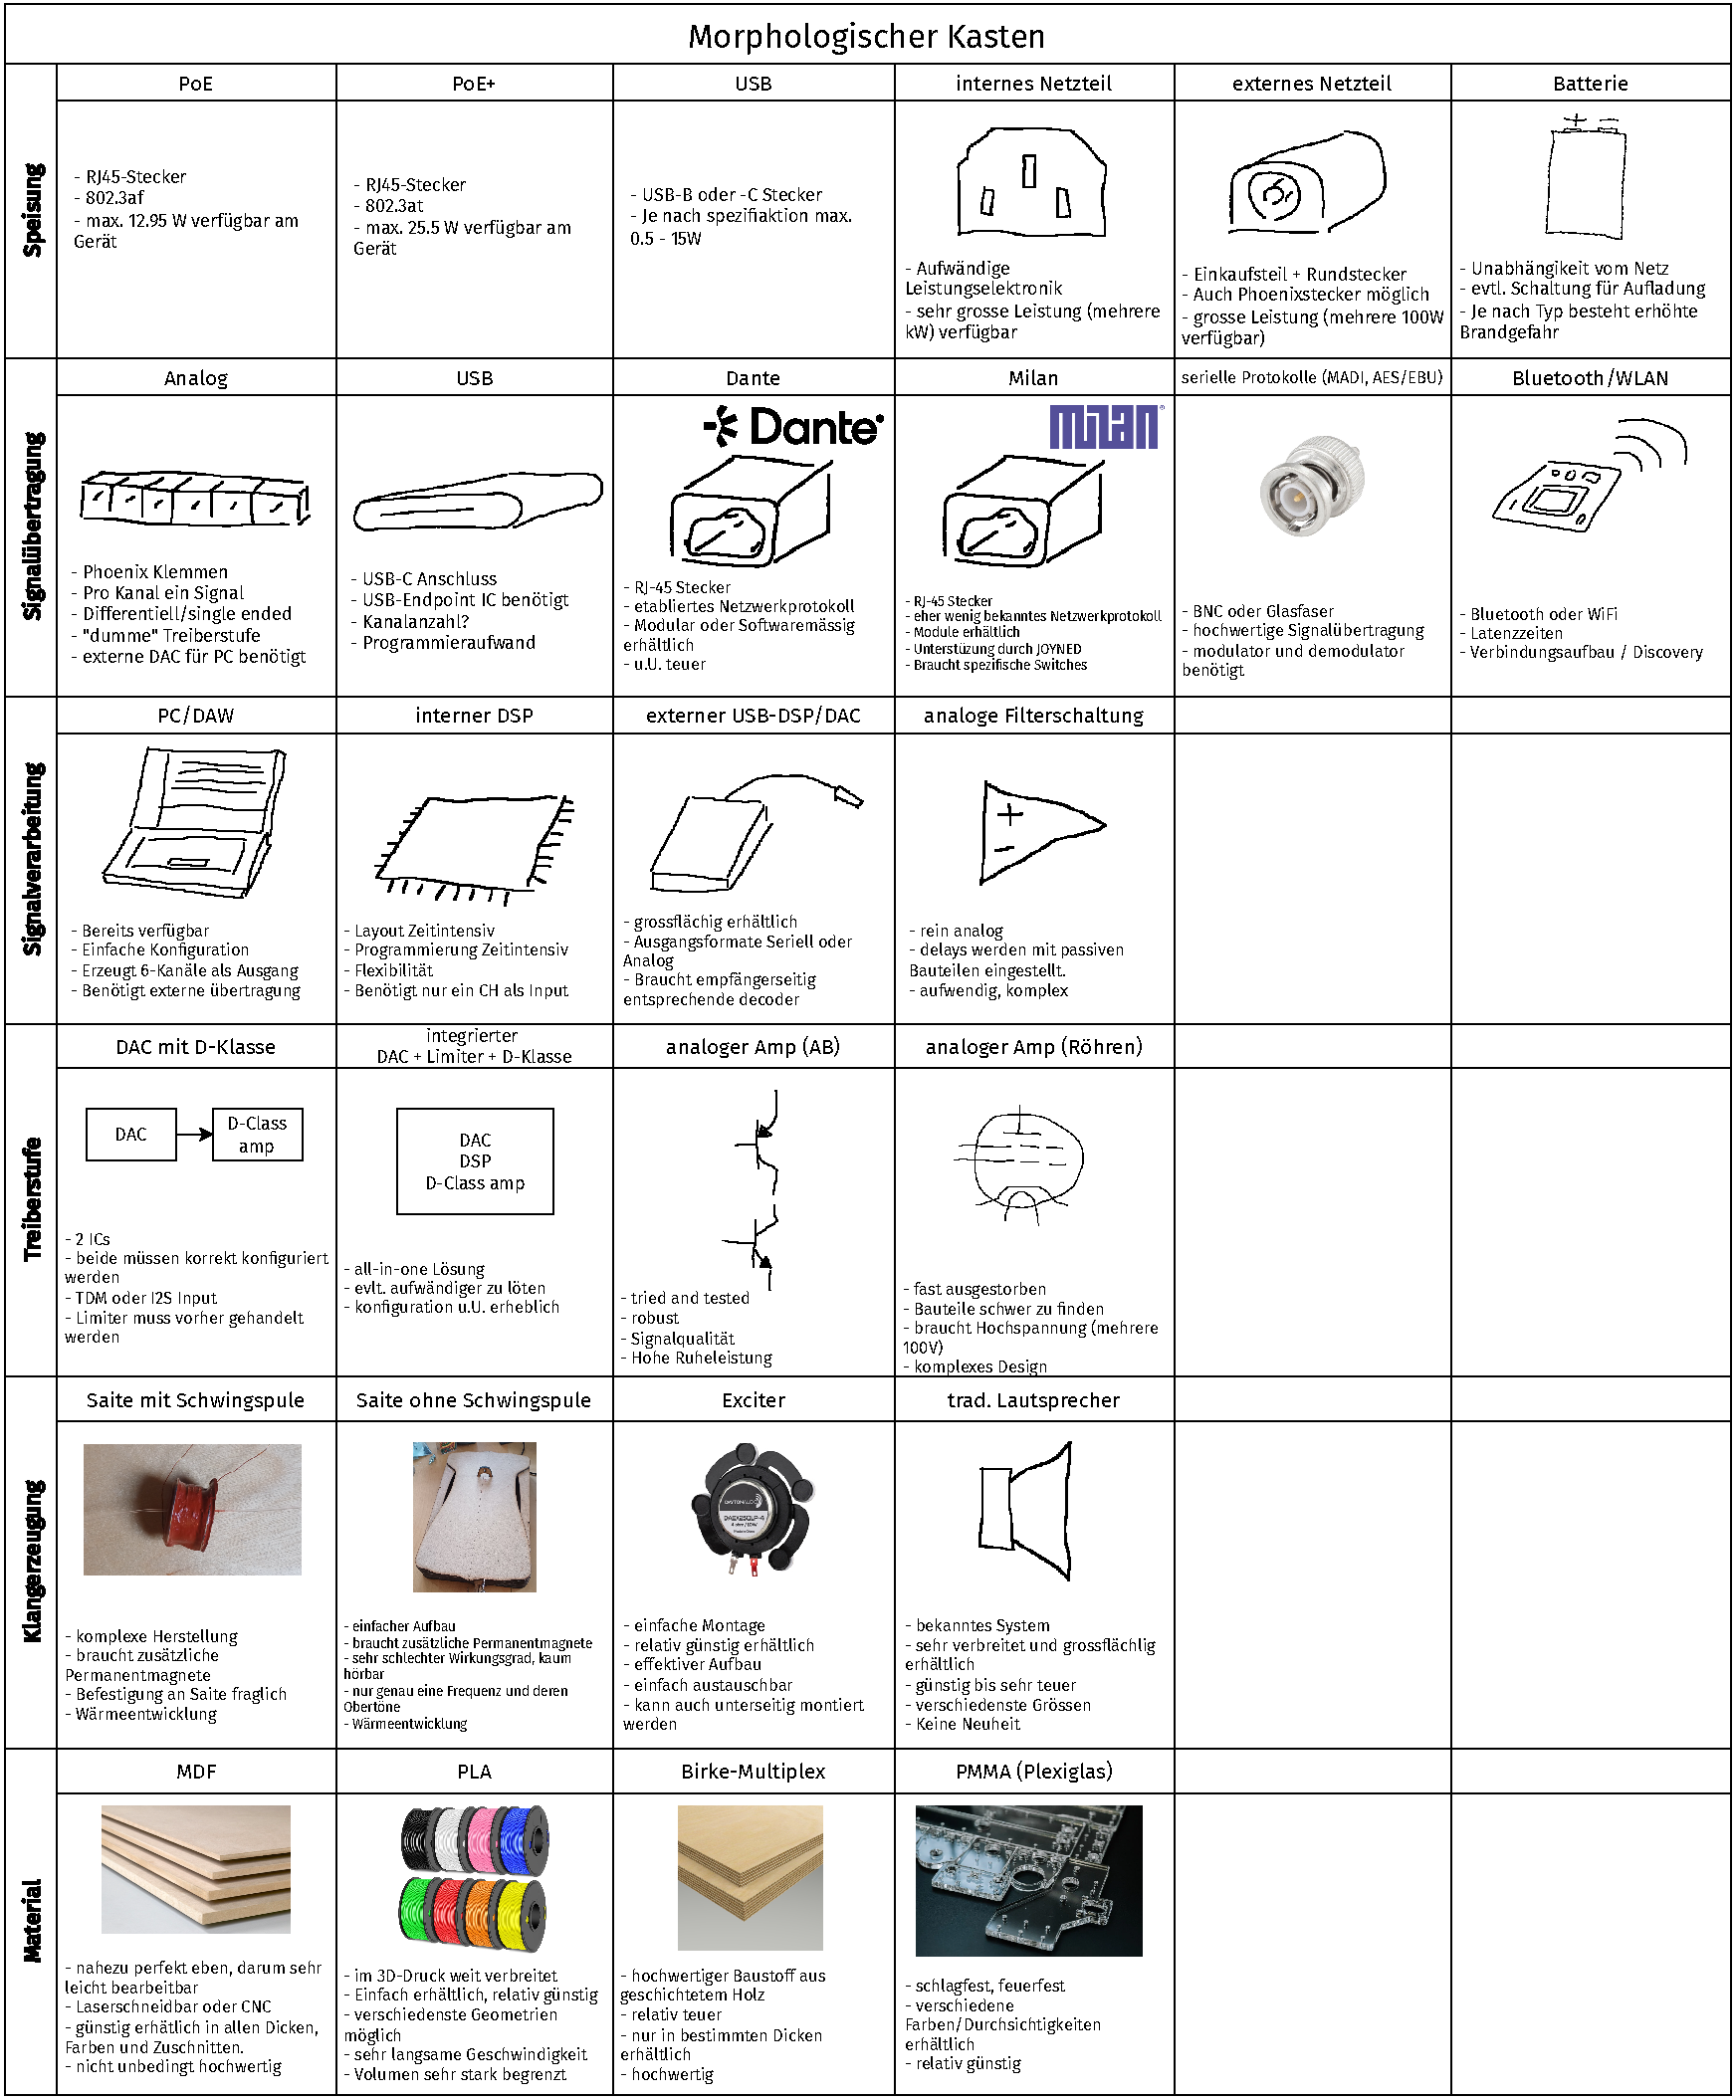
\includegraphics[width=\textwidth]{pictures/morphologischer_kasten.pdf}
	\caption{Der morphologische Kasten}
	\label{pic:morphologischer_kasten}
\end{figure}
\subsubsection{Variante A: Alles Analog}
In dieser Variante wird möglichst alles via analoge Signalpfade geführt. So kann zum Beispiel die Signalverzögerung durch Allpass-Filter realisiert werden. Fokus ist auf Robustheit und Signalreinheit.
\begin{figure}[H]
	\centering
	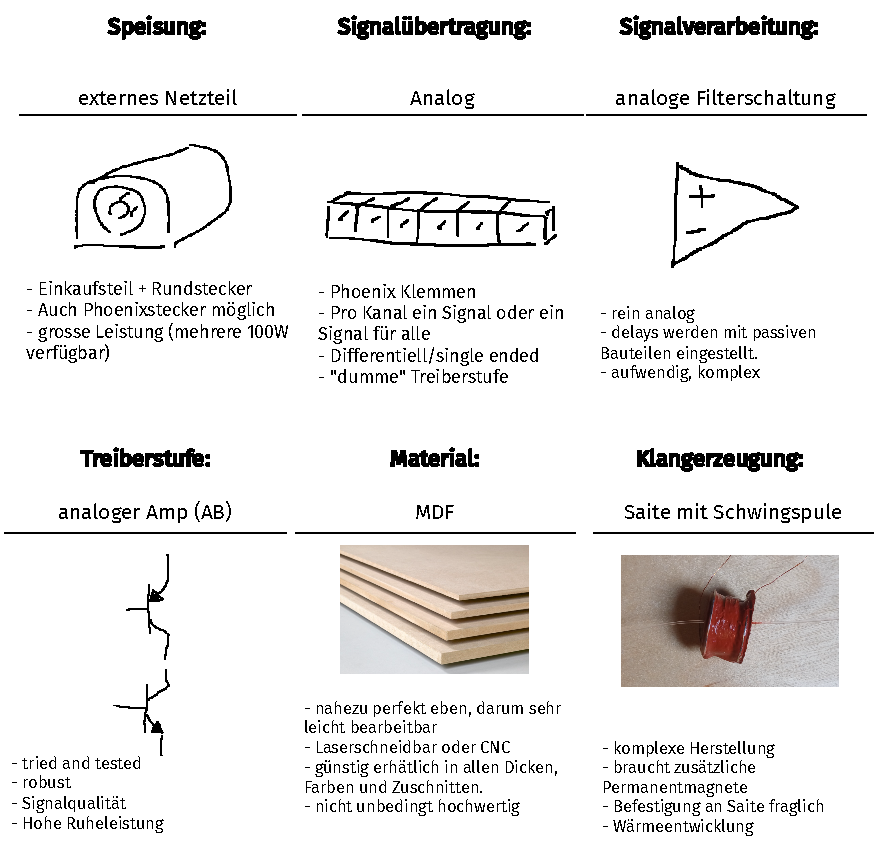
\includegraphics{pictures/VarianteA_allesAnalog.pdf}
	\caption{Variante A}
\end{figure}
\paragraph{Vorteile} Resultate sind relativ schnell messbar. Programmierarbeit erübrigt sich komplett. Zudem sind rein analoge Designs tendenziell robuster und langlebiger. Durch die fehlende Abtastung bleiben Höhenanteile erhalten und die Signalqualität eher hochwertiger.
\paragraph{Nachteile} Fehlersuche ist rein messtechnisch möglich. Nachträgliche Änderungen sehr teuer und Zeitaufwändig. Der Überwachung sind starke Grenzen gesetzt: So muss bei einem Unterbruch der gesamte Signalpfad durchgemessen werden. Ein weiterer Nachteil ist die nur schwer zu realisierende Skalierbarkeit.
\newpage
\paragraph{Risikoanalyse}
Durch sich bewegende Teile, welche unter Umständen durch den Benutzer berührt werden können entsteht zum einen ein Risiko einer leichten Verletzung. Zum anderen könnte die physikalische Montage von analoger Leistungselektronik auf MDF zu einer Brandgefahr führen. Zudem können sehr leicht durch fehlende, unsaubere oder falsche Steckverbindungen Funktionsfehler auftreten.
\begin{figure}[H]
	\centering
	\includegraphics[width=\textwidth*4/5]{pictures/risks-Variante A_ Alles analog.png}
	\caption{Risikoanalyse der Variante A}
\end{figure}
\newpage
\subsubsection{Variante B: Drahtlos \& Portabel}
Der Hauptfokus dieser Variante ist maximale mobilität und minimale Steckverbindungen. Dies wird zum einen durch ein Batterie erreicht, und zum anderen durch eine drahtlose Signalübertragung.
\begin{figure}[H]
	\centering
	\includegraphics{pictures/VarianteB_drahtlosPortabel.pdf}
	\caption{Variante B}
\end{figure}
\paragraph{Vorteile} Da hier die Datenübertragung ohne Stecker auskommt, kann hier im Einsatz komplett auf Kabel verzichtet werden. Somit vereinfachen sich insbesondere weiträumigere Setups, in dem das Gerät weiter weg aufgestellt ist. Als einziger Stecker bleibt ein Ladestecker für die Batterie übrig. Für die Einbindung von Batterien bzw. deren Ladezyklus gibt es zudem bereits sehr viele fertige Komponenten.
\paragraph{Nachteile} Die korrekte Implementierung des Signalpfades von Bluetooth oder Wifi über DSP, den DAC und die D-Klasse Endstufe wird wohl einiges an Aufwand brauchen, insbesondere bei zeitkritischen Anwendungen wie dieser. Zudem entsteht je nach Batterietyp eine Brandgefahr, die zwar durch das Plexiglas vermindert ist aber dennoch z.B. andere Materialien im Raum in Brand setzen kann.
\newpage
\paragraph{Risikoanalyse}
Zwar entfällt hier das Risiko einer falschen Steckverbindung komplett, jedoch erhöht sich durch die Anwesenheit einer Batterie die Brandgefahr deutlich. Dies auch wenn PMMA als Material verwendet wird, da sich die Batterie selbst schon entzünden kann. Zudem entsteht durch den komplexen Aufbau ein unter Umständen zeitintensive Designphase, welche auch mit HF-Layoutfehlern verbunden sein können.
\begin{figure}[h]
	\vspace{1cm}
	\centering
	\includegraphics[width=\textwidth*4/5]{pictures/risks-Variante B_ Portabel und Drahtlos.drawio.png}
	\caption{Risikoanalyse der Variante B}
\end{figure}
\newpage
\subsubsection{Variante C: High-End Audiophil}
Maximale Kontrolle steht bei dieser Variante im Zentrum. Nur bewährte und zuverlässige Komponenten sollen verwendet werden. Einkaufsteile sind nach Verzerrungsfreiheit und rauscharmen Signalpfaden auszuwählen. Preispunkt ist sekundär.
\begin{figure}[H]
	\centering
	\includegraphics{pictures/VarianteC_HighEndAudiophil.pdf}
	\caption{Variante C}
\end{figure}
\paragraph{Vorteile} Die Audioqualität als oberste Priorität begünstigt ein beeindruckendes Hörerlebnis. Zudem ist die Auswahl an bewährten Methoden und robusten Materialien ein Garant für eine lange Lebensdauer.
\paragraph{Nachteile} Als erstes ist hier sicher auch die Komplexität zu nennen, da sehr spezifische Bauteile ausgewählt werden müssen, die unter Umständen nicht weit verbreitet sind. Zum anderen wird hier auch das Budget sehr strapaziert, wohl über die Belastungsgrenzen hinaus.
\newpage
\paragraph{Risikoanalyse}
Die grosse Anzahl verschiedener eigens entworfenen Komponenten führt nebst der Gefahr eines \textit{Scope Creeps} auch eventuell zu Ungenauigkeiten oder unvorhergesehenen negativen Effekten. Zudem kommt zur Leistungselektronik der Endstufe auch die Leistungselektronik des Netzteils hinzu. Auch der Lautsprecher an sich kann überhitzen und zu Brandursachen führen.
\begin{figure}[H]
	\vspace{1cm}
	\centering
	\includegraphics[width=\textwidth*4/5]{pictures/risks-Variante C.png}
	\caption{Risikoanalyse der Variante C}
\end{figure}
\newpage
\subsubsection{Variante D: Einfache Anwendung, Plug'n'Play}
Möglichst einfache Anwendung ist zentral für ein überzeugendes Benutzererlebnis. Daher wurde diese Variante mit diesem Fokus generiert. Zudem ist ein Nebenfokus hier die günstige Herstellung des Systems.
\begin{figure}[H]
	\centering
	\includegraphics{pictures/VarianteD_EinfachPlugnPlay.pdf}
	\caption{Variante D}
\end{figure}
\paragraph{Vorteile} Da Datensignale und Speisung auf einem RJ45-Stecker geliefert werden, muss nur diese eine Verbindung hergestellt werden. Zudem ist mit dem MILAN-Protokoll eine automatische Bandbreitenreservation und somit keine Benutzerkonfiguration notwendig. Da DAC und Treiberstufe in einem Chip integriert ist, bleibt die Programmierung begrenzt. 
\paragraph{Nachteile} Da das Signal direkt vom PC generiert wird, muss dieses zuerst in das MILAN-Protokoll verpackt werden. Zudem muss ein AVB-fähiger Switch verwendet werden.
\newpage
\paragraph{Risikoanalyse}
Die Brandgefahr bleibt nach wie vor ein Hauptfaktor in der Risikoauswertung, bedingt durch die Verbindung von Holzfasern und Leistungsendstufen. Der noch nicht weitum verbreitete MILAN-Standard könnte hier auch zu Inkompatibilitäten, oder zumindest zu einem komplexen Setup führen. Auch könnte die Implementierung eines neuen Standards schnell \textit{Scope Creep} führen, da keine fix fertigen Lösungen bereitstehen.
\begin{figure}[H]
	\vspace{1cm}
	\centering
	\includegraphics[width=\textwidth*4/5]{pictures/risks-Variante D.png}
	\caption{Risikoanalyse der Variante D}
\end{figure}
\newpage
\subsubsection{Variante E: Neu ist besser}
Innovation und moderne Technologie ist das Hauptmerkmal dieser Variante. Es sollen möglichst die neusten Methoden und Komponenten verwendet werden. Etablierte Verfahren sind bereits vollumfänglich im Markt vorhanden und daher uninteressant. Daher werden alles entweder neue Technologien oder bislang nicht verwendete Ideen verwendet.
\begin{figure}[H]
	\centering
	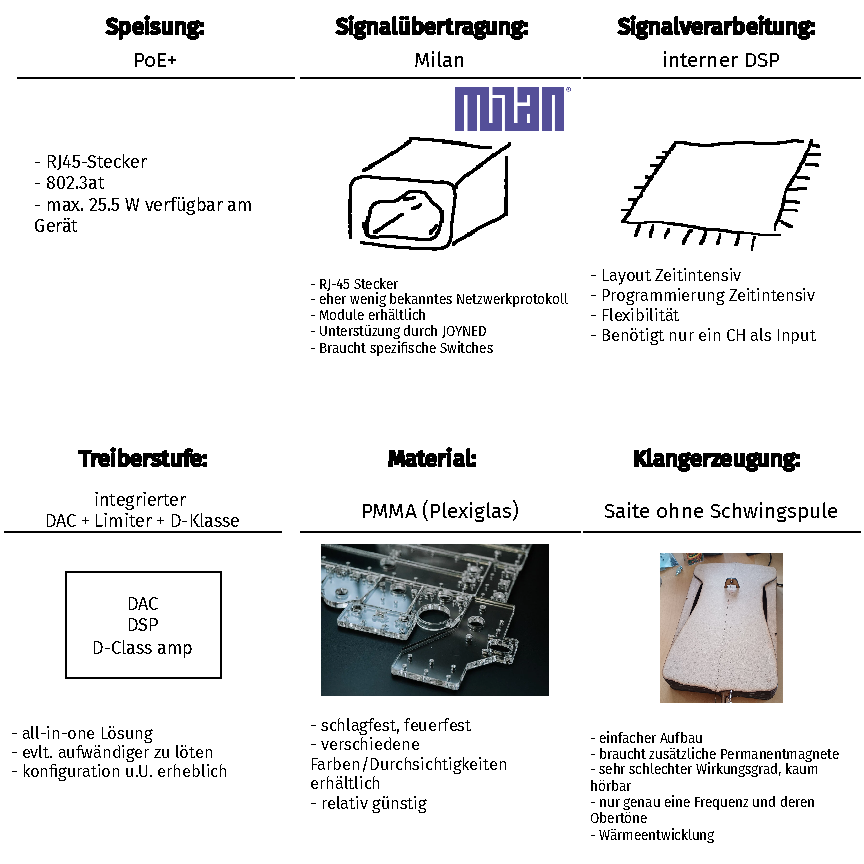
\includegraphics{pictures/VarianteE_Neuistbesser.pdf}
	\caption{Variante E}
\end{figure}
\paragraph{Vorteile} Durch die Neuheit und Innovation entsteht Freiheit: Es gibt in dem Sinne keine etablierte Verfahren oder Protokolle. Daher eröffnet sich ein Spielraum für Eigeninitiative.
\paragraph{Nachteile} Durch die undefinierten Variablen muss sehr viel Arbeit in deren Ausarbeitung investiert werden. So muss die gesamte Signalverarbeitung und die Kommunikation mit dem DAC definiert werden. Zudem entstehen unter Umständen weitere Kosten durch wenig verfügbare Bauteile.
\newpage
\paragraph{Risikoanalyse}
Nebst hohen Herstellungskosten kann hier eine stromdurchflossene Saite erhitzen und zu Verbrennungen führen. Des weiteren kann die Impedanz der Saite schlicht zu tief sein für die Endstufe, wodurch die Schwingung wenn überhaupt nur kaum wahrnehmbar also extrem leise erzeugt werden kann. Zudem entsteht durch den internen DSP auch hier die Gefahr des \textit{Scope Creep}, da die Signalverarbeitung potentiell recht umfangreich werden kann.
\begin{figure}[H]
	\vspace{1cm}
	\centering
	\includegraphics[width=\textwidth*4/5]{pictures/risks-Variante E.png}
	\caption{Risikoanalyse der Variante E}
\end{figure}
\newpage
\section{Variantenauswertung}
\subsubsection{Nutzwertanalyse}Zur Auswertung wurde eine Nutzwertanalyse durchgeführt, bei der die Primärkriterien auf Erfüllung oder Nichterfüllung hin geprüft wurden. Idealerweisen sollten dabei alle Primärziele erfüllt werden. Alle anderen Ziele wurden gemäss Tabelle \ref{tab:zielgewichtung} neu gewichtet und deren Erfüllung mit einer Note von 1 bis 10 und bei Nichterfüllung 0 bewertet. Die Multiplikation der Gewichtuung mit der Note ergibt ein Zwischenresultat für ein Ziel. Die Summe der Zwischenresultate ergibt die Gesamtpunktzahl nach Sekundärzielen. Diese Analyse ist in Abbildung \ref{pic:nutzwertanalyse} dargestellt. Mit diesen Kriterien erfüllt nur \textbf{Variante D} die Muss-Ziele.
\subsubsection{Kosten-Nutzen Analyse}
In Bezug zu den verwendeten Komponenten und Materialien kann eine Schätzung für die Kosten jeder Variante abgegeben werden:
\begin{itemize}
	\item \textbf{Variante A: Alles Analog}: Hoch, vor allem durch den Zeitaufwand
	\item \textbf{Variante B: Drahtlos \& Portabel}: Mittel, jedoch PMMA als Preistreiber
	\item \textbf{Variante C: High-End Audiophil}: Sehr hoch, durch Spezial- und High-End Komponenten
	\item \textbf{Variante D: Einfache Anwendung, Plug’n’Play}: Tief-Mittel
	\item \textbf{Variante E: Neu ist besser}: Mittel, jedoch PMMA und Zeitaufwand
\end{itemize}
Diese Erkenntnis kann auf die in der Nutzwertanalyse erreichte Punktzahl abgebildet werden. Abbildung \ref{pic:kostennutzen} zeigt dieses Verhältnis grafisch auf. Dabei sind Lösung mit Tendenz in Richtung untere rechte Ecke (\textit{hoher Nutzen, tiefe Kosten}) zu bevorzugen. Dagegen sind Lösungen mit Tendenz Richtung oberen linke Ecke mit hohen Kosten, aber wenig Nutzen verbunden.
\begin{figure}[H]
	\centering
	\includegraphics[width=\textwidth - 2cm]{pictures/Kostennutzenanalyse.png}
	\caption{Kosten-Nutzen Analyse}
	\label{pic:kostennutzen}
\end{figure}
\newpage
\begin{figure}[H]
	\centering
	\includegraphics[trim={0 3cm 0 0},clip,width=\textheight - 1cm, angle=90]{pictures/Nutzwertanalyse.pdf}
	\caption{Nutzwertanalyse}
	\label{pic:nutzwertanalyse}
\end{figure}
\newpage
\section{Variantenauswahl}
Die Variantenanalysen zeigt klar, dass \textbf{Variante D: Einfache Anwendung} aus Risikogründen, Nutzwertanalyse und der Kosten-Nutzen die vielversprechendste Variante ist. Die Kombination aus fixfertigen Modulen, wenigen Neuentwicklungen und wenigen Komponenten führt in vielen Belangen zu vorteilhaften Eigenschaften. Ein weiterer Vorteil ist, dass durch den Einsatz von Excitern sich die Konstruktion erheblich vereinfacht, da keine Saite gespannt oder fixiert werden muss und keine sich bewegende Teile von aussen zugänglich sind.

%
%\paragraph{Anpassungen}Nichtsdestotrotz kann diese Variante noch weiter optimiert und kombiniert werden. So können zum Beispiel mehrere Materialien für das Gehäuse verwendet werden. Daher wurde diese Variante auf die Primärziele hin noch weiter angepasst. Nachfolgend sind daher die Primärziele mit den entsprechenden Massnahmen aufgelistet:\\
%\begin{figure}[H]
%	\centering
%	\setstretch{1.5}
%	\begin{tabularx}{\textwidth*4/5}{lX}
%		{\large \textbf{Ziel}} & {\large Massnahme}\\
%		\midrule\vspace{-6mm}\\
%		\textbf{G: Reduziertes Brandrisiko}&Montage der stromführenden Bauteile auf PMMA\\
%		\vspace{2mm}\textbf{D.2: Mobilität}&Einsatz eines externen USB-MILAN Dongles für die Verbindung zwischen PC und Gerät. Somit ist kein Switch vonnöten.\\
%		\vspace{2mm}\textbf{A: Direktionale Abstrahlung}&Externes Netzteil für grösseres Leistungsbudget\\
%		\bottomrule
%	\end{tabularx}
%	\caption{Weitere Massnahmen}
%\end{figure}


\section{Terminplanung}
Für das Projekt wurden nun abgegrenzte Arbeitspakete definiert und diese in einen Zeitplan überführt. Dabei wurde darauf geachtet, dass wichtigere bzw. kritische Pakete (z.B. die Variantenauswahl) mehr Zeit bekamen. Als Hilfmittel wurde zudem die Projektfunktion von github.com verwendet. Dieses Tool bietet nicht nur den Vorteil einer grafischen Darstellung (Roadmap, Burn-up etc.), sondern auch dass jedes Paket mit einer Historie, Kommentaren (auch von dritten), Files, Links sowie Referenzen untereinander ergänzt werden. So kann der Projektverlauf dynamisch auf jedes einzelnes Paket hin verfolgt werden.\\In Tabelle \ref{terminplan} sind alle Arbeitspakte, deren Zeitrahmen sowie den jeweiligen Github-Links nochmals tabellarisch dargestellt.
\begin{table}[H]
	\centering
	\caption{Terminplanung in tabellarischer Form}
	\setstretch{1.5}
	\begin{tabularx}{412pt}{|l|l|l|l|}
		\textbf{Arbeitspaket} & \textbf{URL} & \textbf{Startdatum} & \textbf{Enddatum} \\\hline
		\textbf{Terminplanung} & \href{https://github.com/Violabitch5/Nathophone\_doc/issues/1}{Link} & Sep 4, 2025 & Sep 5, 2025 \\ 
		\textbf{IST-Zustandsanalyse} & \href{https://github.com/Violabitch5/Nathophone\_doc/issues/4}{Link} & Sep 6, 2025 & Sep 7, 2025 \\ 
		\textbf{Zieldefinition} & \href{https://github.com/Violabitch5/Nathophone\_doc/issues/3}{Link} & Sep 8, 2025 & Sep 9, 2025 \\ 
		\textbf{Zielgewichtung} & \href{https://github.com/Violabitch5/Nathophone\_doc/issues/5}{Link} & Sep 10, 2025 & Sep 11, 2025 \\ 
		\textbf{Varianten- \& Risikoanalyse} & \href{https://github.com/Violabitch5/Nathophone\_doc/issues/6}{Link} & Sep 12, 2025 & Sep 16, 2025 \\ 
		\textbf{Variantenauswahl} & \href{https://github.com/Violabitch5/Nathophone\_doc/issues/7}{Link} & Sep 17, 2025 & Sep 17, 2025 \\ 
		\hdashline
		\textbf{Kennzahlberechnung / Limits} & \href{https://github.com/Violabitch5/Nathophone\_elec/issues/1}{Link} & Sep 18, 2025 & Sep 21, 2025 \\ 
		\textbf{Bauteileevaluation} & \href{https://github.com/Violabitch5/Nathophone\_elec/issues/2}{Link} & Sep 22, 2025 & Sep 30, 2025 \\ 
		\textbf{Bauteilauswahl} & \href{https://github.com/Violabitch5/Nathophone\_elec/issues/3}{Link} & Oct 1, 2025 & Oct 4, 2025 \\ 
		\textbf{Print Schema draft} & \href{https://github.com/Violabitch5/Nathophone\_elec/issues/4}{Link} & Oct 5, 2025 & Oct 11, 2025 \\ 
		\textbf{Print Schema v1} & \href{https://github.com/Violabitch5/Nathophone\_elec/issues/5}{Link} & Oct 12, 2025 & Oct 18, 2025 \\ 
		\textbf{Print Layout v1} & \href{https://github.com/Violabitch5/Nathophone\_elec/issues/6}{Link} & Oct 19, 2025 & Oct 26, 2025 \\ 
		\textbf{Peer-review Schema und Layout} & \href{https://github.com/Violabitch5/Nathophone\_elec/issues/7}{Link} & Oct 27, 2025 & Oct 31, 2025 \\ 
		\textbf{Print Schema Final} & \href{https://github.com/Violabitch5/Nathophone\_elec/issues/8}{Link} & Nov 1, 2025 & Nov 3, 2025 \\ 
		\textbf{Print Layout final} & \href{https://github.com/Violabitch5/Nathophone\_elec/issues/9}{Link} & Nov 3, 2025 & Nov 6, 2025 \\ 
		\textbf{Gerber-Daten generieren und Printbestellung} & \href{https://github.com/Violabitch5/Nathophone\_elec/issues/10}{Link} & Nov 7, 2025 & Nov 7, 2025 \\ 
		\textbf{Konstruktion des Korpus fertigstellen} & \href{https://github.com/Violabitch5/Nathophone\_mech/issues/1}{Link} & Nov 8, 2025 & Nov 10, 2025 \\ 
		\textbf{Herstellung Korpus-Teile} & \href{https://github.com/Violabitch5/Nathophone\_mech/issues/2}{Link} & Nov 11, 2025 & Nov 15, 2025 \\ 
		\textbf{Zusammenbau Korpus} & \href{https://github.com/Violabitch5/Nathophone\_mech/issues/3}{Link} & Nov 16, 2025 & Nov 22, 2025 \\ 
		\textbf{Bestückung + Lötarbeit Print} & \href{https://github.com/Violabitch5/Nathophone\_elec/issues/11}{Link} & Nov 23, 2025 & Nov 30, 2025 \\ 
		\textbf{Funktionstest Print} & \href{https://github.com/Violabitch5/Nathophone\_elec/issues/12}{Link} & Dec 1, 2025 & Dec 4, 2025 \\ 
		\textbf{Zusammenbau Komplettsystem \& Programmierung} & \href{https://github.com/Violabitch5/Nathophone\_mech/issues/4}{Link} & Dec 4, 2025 & Dec 18, 2025 \\ 
		\textbf{Funktionstests Komplettsystem} & \href{https://github.com/Violabitch5/Nathophone\_elec/issues/13}{Link} & Dec 18, 2025 & Dec 25, 2025 \\ 
		\textbf{Schlussmessung \& Auswertungen} & \href{https://github.com/Violabitch5/Nathophone\_elec/issues/14}{Link} & Dec 25, 2025 & Dec 31, 2025 \\ 
		\hdashline
		\textbf{Audruck (Plakat und Arbeit)} & \href{https://github.com/Violabitch5/Nathophone\_doc/issues/8}{Link} & Jan 1, 2026 & Jan 6, 2026 \\ 
		\textbf{Abgabe Diplomarbeit} & \href{https://github.com/Violabitch5/Nathophone\_doc/issues/2}{Link} & Jan 7, 2026 & Jan 7, 2026
	\end{tabularx}
	\label{terminplan}
\end{table}
\vspace{-4mm}
%--- Theory -------------------------------------

%--- Umsetzung -----------------------------------------
\chapter{Umsetzung}
\section{Blockschaltbild}
Mit der erarbeiteten Variante aus dem System Engineering wurde nun ein Blockschaltbild erstellt. Dieses ist in Abbildung \ref{pics:blockschaltbild} dargestellt. In diesem wurden bereits einige Komponenten ausgewählt: 
\paragraph{MILAN Modul MT32-TDM to MILAN} Die Firma \href{https://www.joyned.at/}{JOYNED GmbH} bietet auf ihrem Webshop bereits ein fix-fertiges Milan-Modul an, welches über PoE gespiesen wird und 16x16 Audiokanäle verarbeiten kann (siehe \cite{joyned_store}). Abbildung \ref{pics:mt32_TDM} zeigt das Modul. Zum Anschluss in einem Gerät dient ein System Connector, welches nebst den Datensignalen in TDM-Format (\textbf{Time Division Multiplex}) auch Master Clock-, I$^{2}$C-, GPIO-, 3V- und 5V-Leitungen besitzt.
\begin{figure}[H]
	\centering
	\includegraphics[width=\textwidth*3/4]{pictures/Joyned_MT32-TDM.png}
	\caption{Das Milan-Modul der Firma Joyned GmbH}
	\label{pics:mt32_TDM}
\end{figure}
\paragraph{Gehäuse}Das Gehäuse wurde schon in der Vorarbeit gezeichnet und war daher schon gegeben. Auf einem länglicher Resonanzkasten sind sechs Membran-Platten angebracht, die unabhängig voneinander in Schwingung gebracht werden können. Zusätzlich ist auch eine Aussparung für die Elektronik vorgesehen. Abbildung \ref{pics:render_box} zeigt eine grafische Darstellung davon.
\begin{figure}[H]
	\centering
	\includegraphics[width=\textwidth]{pictures/Nathophone_2025-Sep-29_07-57-22AM-000_CustomizedView2892546826.png}
	\caption{Das Gehäuse mit 6 Frontplatten}
	\label{pics:render_box}
\end{figure}
\begin{figure}[H]
	\centering
	\includegraphics[width=\textwidth]{pictures/blockschaltbild.pdf}
	\caption{Das Blockschaltbild}
	\label{pics:blockschaltbild}
\end{figure}
Bei der Erstellung wurde schnell klar, dass auch noch einige undefinierte Komponenten vorhanden waren. So musste noch bestimmt werden, was von wo gespiesen werden soll.
\\Zudem war noch unklar, ob der USB-Milan Dongle direkt auf das Modul verbunden werden kann (evtl. über einen PoE-Injector\footnote{Ein Gerät, welches einer Ethernet-Verbindung eine PoE-Speisespannung hinzufügt und seriell in die Verbindung geschaltet wird.}) oder über einen Milan-fähigen Switch verbunden werden muss.
\\Des weiteren war noch nicht klar, ob nebst den Datenleitungen des Moduls (Serial Audio Interface und I2C) auch noch die anderen Signale wie Master Clock etc. verwendet werden müssen.
\\Als letzter Punkt musste noch abgeklärt werden, ob das Modul zwingend mit PoE, oder ob auch über den System Connector gespiesen werden kann. Also 3V- und 5V-Pins als Eingänge.
\section{Kennzahlen}
\subsection{Leisungsbudget}
Somit lagen bereits einige Kennzahlen vor, die eingehalten werden mussten:
\paragraph{Anzahl Exciter: 6} Dies ist durch den Korpusaufbau gegeben. Eine höhere Anzahl hätte zwar akustisch einige Vorteile, ist aber mit grösseren Dimensionen und/oder höheren Kosten verbunden.
\paragraph{Leistung (Continous) pro Exciter: 0.5 bis 150 Watt} Dies sind zunächst der Bereich der Leistungskennzahlen aller verfügbaren Exciter auf \href{https://www.soundimports.eu/en/audio-components/exciters/?hr-page=%7B%22page%22%3A1%2C%22active_filter%22%3A%22%22%2C%22filters%22%3A%5B%5D%2C%22product_count%22%3A0%7D}{soundimports.eu}. Da die grösseren Excitermodelle oft für Kino-Effekte wie z.B. Vibrationen des Tyrannosaurus Rex verwendet werden, gibt es entsprechende Modelle für Bassfrequenzen mit Leistungsangaben bis 150W. Da bei dieser Arbeit das Ziel einer möglichst tiefen Grenzfrequenz nicht im Vordergrund stand (siehe \nameref{sec:zielgewichtung}), kamen wesentlich kleinere Modelle für die Exciter in Frage. Zu den Leistungskennzahlen allerdings noch ein kurzer Einschub, da diese immer wieder zu Missverständnissen führen:
\subsubsection{Leistungsangaben bei Lautsprechern} \label{chap:leistungsangaben} In der Audioindustrie werden in der Regel mindestens drei Kennzahlen für die Maximalleistung eines Lautsprechers genannt:
\begin{itemize}
	\item \textbf{RMS Power Handling\footnote{Im Grunde genommen ist der Effektiv- oder RMS-Wert einer Leistung keine Sinnvolle Angabe: Der Effektivwert eines Strom- und Spannungssignals wird nur genutzt, um die durchschnittliche Leistung zu berechnen. Der RMS-Wert eines Leistungssignals hat somit eigentlich keinen weiteren Nutzen.}} oder auch \textbf{Continuous Power} oder auch \textbf{Rated Noise Power}
	\item \textbf{Power(Programm)} oder auch \textbf{Rated Power}
	\item \textbf{Peak Power} oder auch \textbf{Power handling Peak}
\end{itemize}
Diese Begriffe werden teilweise sehr unterschiedlich verwendet, bisweilen auch vom selben Hersteller. Es ist am einfachsten, beim letzten Begriff zu beginnen:
\textbf{Peak Power} beschreibt die absolut maximale Leistung, die ein Lautsprecher zu einem einzelnen Zeitpunkt noch verträgt. Also führt einem Signal mit einem 1mW höheren Spitzenwert (theoretisch) zur Zerstörung des Produkts.\\Der Peak-Wert wird nun als Ausgangsbasis verwendet, um die durchschnittliche kontinuierliche Leistung zu berechnen, die der Lautsprecher über längere Zeit\footnote{meist eine Stunde} noch aushält. Diese maximale Durschnittsleistung hängt allerdings stark vom Crest-Faktor, also dem Verhältnis zwischen Spitzen- und Effektivwert eines Signals, ab. Die \citetitle{aespar} der Acoustic Engineering Society (AES)  erläutert den Begriff:
\begin{quotation}
	\textbf{crest factor} The term used to represent the ratio of the peak (crest) value to the rms value of a waveform measured over a specified time interval. For example, a sine wave has a crest factor of 1.4 (or 3 dB), since the peak value equals 1.414 times the rms value. Music has a wide crest factor range of 4-10 (or 12-20 dB) [\textit{Hier wird in Volt, also 6dB pro Verdopplung gerechnet.}]. This means that music peaks occur 12-20 dB higher than the rms value, which is why headroom is so important in audio design.\\Quelle: \cite{aespar} \label{cite:crest}
\end{quotation}
%\begin{quotation}
%	As we've mentioned, pink noise can have various crest factors, but the crest factor in testing is typically 2 [\textit{Spannungsbezogen}].\\Quelle: \cite{SoundreinforcementforaudioEngineers}
%\end{quotation}
In der Praxis wird also ein Testsignal\footnote{gemäss IEC 60268-1:1985} verwendet, welches typischerweise einen Crest-Faktor von 6dB (Leistungsbezogen) hat. Somit ist der Wert für \textit{RMS Power Handling} oder \textit{Cont. Noise Power} 4-mal tiefer als der Peak Wert.
\subsubsection{Endstufenleistung}\label{subsection:Theory_ampgain}Die Endstufe muss diese Leistung des Lautsprechers auch tatsächlich liefern können. Andernfalls wird die in vielen Endstufen vorhandene Leistungsbegrenzung (eng. \textit{Limiter}) aktiviert und somit bei Vollausschlag eine Gleichspannung erzeugt, welche die Schwingspule im Lautsprecher maximal stark auf eine Seite hin auslenkt und somit den Lautsprecher beschädigen oder gar zerstören kann. Die Endstufe muss also mindestens die nominale Cont.-Leistung des Lautsprechers liefern können. In der Praxis wird als Faustregel für die Endstufenleistung die doppelte Cont.-Leistung des Lautsprechers empfohlen, damit die Endstufe auch alle Signalspitzen gut abbilden kann. Durch digitale Limiter-Presets, welche Grenzwerte für Cont. und Peak enthalten, kann der Schutz des Lautsprechers sichergestellt werden. 
Abbildung \ref{pics:adc820_pwr} zeigt diese Angaben aus einem Datenblatt eines Deckeneinbaulautsprechers (\cite{adc820man}). Jedoch wird keine Peak-Leistung angegeben. Abbildung \ref{pics:adc820_footnote} zeigt die Fussnoten, welche einen Crestfaktor von 6dB angeben.
\begin{figure}[H]
	\centering
	\includegraphics[width=\textwidth*5/9]{pictures/adc820_pwr.png}
	\caption{Leistungsangaben eines Deckenlautsprechers, ohne Peak Power}
	\label{pics:adc820_pwr}
\end{figure}
\begin{figure}[H]
	\centering
	\includegraphics[width=\textwidth*5/9]{pictures/adc820_footnotes.png}
	\caption{In den Fussnoten findet sich der Crest-Faktor}
	\label{pics:adc820_footnote}
\end{figure}
\subsubsection{Entscheid Exciterleistung}
Aus den Vorarbeiten ging heraus, dass bereits ein Excitermodell mit 10W Cont.-Leistung extrem Effizient und weitaus höhere Schallpegel erzeugt als in dieser Anwendung erfordert. Der dabei verwendete Exciter war ein \textbf{DAEX25QLP-4} von Dayton Audio. Abbildung \ref{pics:DAEX25QLP4_freqresp} zeigt den Frequenzgang dieses Modells. Dieser bewegt sich durchschnittlich im Bereich von 75-80 dB SPL\footnote{Eine SPL-Nominalwert wird im Datenblatt nicht angegeben. Zudem fehlt die Angabe ob A-, B- oder Z-Gewichtet wurde}. Der Vergleich mit dem kleineren Modell \textbf{DAEX19QLP-4} (Abbildung \ref{pics:DAEX19QLP4_freqresp}) zeigt, dass dieser im Bereich von 100-1000Hz zwar ca. 5 dB weniger Pegel erzeugt, darüber sogar noch einen lineareren Frequenzgang aufweist.\\
\begin{center}
	\begin{minipage}{\textwidth*7/8}
		\centering
		{\large Aus dieser Beobachtung wurde geschlossen, dass auch ein \textbf{Exciter mit 5W Cont.} bereits für diese Anwendung ausreicht.}
		\vspace{6mm}
	\end{minipage}
\end{center}
Aus Zeitgründen und um genug Headroom für hohe Signalpegel zu haben, wurde darauf verzichtet, noch kleinere Leistungsmodelle zu evaluieren.
\begin{figure}[H]
	\centering
	\includegraphics[width=\textwidth*7/8]{pictures/DAEX25QLP4_freqresp.png}
	\caption{Quelle: \cite{DAEX25QLP4spec}}
	\label{pics:DAEX25QLP4_freqresp}
\end{figure}
\begin{figure}[H]
	\centering
	\includegraphics[width=\textwidth*7/8]{pictures/DAEX19QLP4_freqresp.png}
	\caption{Quelle: \cite{DAEX19QLP4spec}}
	\label{pics:DAEX19QLP4_freqresp}
\end{figure}
\subsubsection{PoE}
In der Netzwerktechnik als weit verbreiteter Standard zur gleichzeitigen Übertragung von Speisung und Daten etabliert, bietet PoE (\textit{Power over Ethernet}) eine extrem einfache und attraktive Lösung für dieses Projekt. Jedoch hat der Standard auch einige Tücken, und gerade die höheren Leistungsklassen (PoE++) können schnell extrem kostenintensiv werden. Zudem hängt das ganze nochmals vom verwendeten Kabel, und dessen Querschnitt ab. Abbildung \ref{pic:poe_overview} zeigt eine anschauliche Übersicht über den Standard und die verfügbaren Leistungen (Quelle: \cite{PoE_overview_doc}).
\begin{figure}[H]
	\centering
	\includegraphics[width=\textwidth*3/4]{pictures/PoE_overview.png}
	\caption{Eine Übersicht über die PoE-Klassen}
	\label{pic:poe_overview}
\end{figure}
\subsubsection{Gesamtes Leisungsbudget}
Mit dem Wissen aus \ref{chap:leistungsangaben} konnte nun eine Aussage über die voraussichtlich benötigte Nominalleistung der Endstufe und der Speisung gemacht werden. Zu beachten war hier, dass die gesamte Endstufe sechs Kanäle enthält, die (ideale) Gesamtleistung sechs mal der Leistung eines Kanals entspricht. In einer Grafik konnten nun alle Leistungswerte als Balken dargestellt und verglichen werden (Abbildung \ref{pic:Leistungsbudget}). Darin sind zum Vergleich auch die am Gerät verfügbaren Nennleistungen der PoE-Klassen (PoE, PoE+ und PoE++). Es zeigt sich somit, dass auch die höchste PoE-Klasse nur sehr knapp die geforderte Gesamtleistung für sechs Kanäle zu erbringen vermag (bzw. nur mit einem sehr aufwändigem Puffer) und daher als alleinige Speisung für das komplette Gerät nicht infrage kommt. Die Stromaufnahme des Milan-Moduls betrug laut Herstellerangaben zwischen 350-500mA, also 1.75-2.5W bei 5V. Diese Leistung ist relativ gering im Vergleich zu den Endstufenkanälen.
\begin{figure}[H]
	\centering
	\includegraphics[width=\textwidth]{pictures/Leistungsbudget.pdf}
	\caption{Das Leistungsbudget}
	\label{pic:Leistungsbudget}
\end{figure}

\section{Bauteilevaluation}
Gemäss dem Blockschaltbild (Abbildung \ref{pics:blockschaltbild}) mussten also hauptsächlich zwei noch unbekannte Komponenten definiert werden: \textbf{Die Endstufe(n)} und \textbf{die Speisungsregelung}.
\subsection{Evaluation der Endstufe(n)}
Es blieb zu wenig Zeit, um die tausenden verfügbaren Endstufen einzeln zu evaluieren. Deshalb wurde hier mit ChatGPT eine AI eingesetzt, welche mit folgendem Prompt getriggert wurde:\\
\begin{center}
	\begin{parbox}[][][]{\textwidth*3/4}
		{\textit{\dotfill\\recommend me some D-Class loudspeaker driver chips which can handle at least 7.5 Watts and accepts digital inputs such as I2S or TDM and has an integrated limiter}\\.\dotfill.}
	\end{parbox}
\end{center}\vspace{3mm}
Die Antwort der KI war:\\.\dotfill.\\\textit{\textbf{{\Large Recommendations (short list})}\\
	1) \textbf{TAS2770 (TI)} — Mono, 20 W class-D, digital in, speaker-protection / peak limiter
	\\Power: up to 20 W (mono) (depends on VDD and load).\\Digital input: I2S/TDM compatible (host supplies I2S / TDM).\\Limiter/protection: built-in speaker voltage \& current sensing and a battery-tracking peak-voltage limiter / SmartAmp style protections.\\Supply: 4.5–18 V (check datasheet graphs for exact conditions).\\Good for: battery-powered speakers, portable devices where speaker protection \& headroom tracking matter.\\2) \textbf{TAS5720 / TAS5720x (TI)} — Mono, ~20 W class-D, digital/TDM input, protection features\\Power: ~20 W (mono) (VDD and load dependent).\\Digital input: supports I2S / TDM (up to multi-device arrays).\\Limiter/protection: includes speaker protection and status/diagnostics; datasheet describes the SAIF serial audio interface and protection features.\\Supply: 4.5–26.4 V (device variant dependent).\\Good for: simple mono modules and multichannel TDM systems.\\3) \textbf{TAS5760 / TAS5760L(TI)} — Stereo, closed-loop digital-in Class-D, integrated digital clipper/limiter\\Power: stereo ≈21 W / ch (mono bridged higher) depending on supply/impedance.\\Digital input: native I2S input (digital-in family).\\Limiter/protection: integrated digital clipper / closed-loop speaker sensing and diagnostic features.\\Supply: ~4.5–16 V (variant dependent).\\Good for: stereo compact systems that need closed-loop control and built-in clipping/limiting. 
	Texas Instruments\\4) \textbf{TAS2781 (TI)} — Mono digital-in SmartAmp, ~25 W, integrated speaker-protection \& real-time algorithms\\Power: ~25 W (mono) (depends on supply and load).\\Digital input: I2S from host; integrated DSP for processing and protection.\\Limiter/protection: TI “SmartAmp” speaker protection algorithms and I/V sense for real-time protection.\\Supply: 4.5–23 V.\\Good for: louder mono drivers where sophisticated protection and DSP control are wanted.\\5) \textbf{TAS2557 / TAS255x family (TI)} — Integrated DAC + Class-D with SmartAmp protection (lower power members available ~5–10 W up to bigger SoCs)\\Power: some family members are in the >7.5 W range (check exact part variant).\\Digital input: on-chip DAC + I2S input.\\Limiter/protection: TI SmartAmp/clipper features, speaker sensing on higher-end members.\\Good for: integrated DAC + amp single-chip solutions for compact designs.\\6) \textbf{SSM3515 (Analog Devices)} — Mono digital-input Class-D, up to ~25–31 W (depending on VDD \& load), with AGC/limiting features\\Power: datasheet shows ~25–31 W under certain VDD / load / THD conditions (check graphs).\\Digital input: supports digital audio interface; I2C control for gain/setting.\\Limiter/protection: supply-monitoring AGC function and other protection features (useful as a limiter/level control).\\Good for: applications needing a digital-in amp with AGC/limiting.}\\.\dotfill.\\
\subsubsection{Kurzevaluation}Obwohl die KI anscheinend bevorzugt die grösseren Hersteller (Texas Instruments und Analog Devices) auflistet und hier eher TI-Produkte auswählt, wurde die Antwort als wertvoller Input angesehen. Nach einer kurzen Recherche wurde klar, dass einige bereits ältere Modelle vorgeschlagen wurden. Jedoch haben sich bei genauerer Evaluation zwei Modelle als potentiell Interessant für dieses Projekt erwiesen: Der TAS2781 und TAS5720. Abbildungen \ref{pic:blockschaltbild_TAS2781} und \ref{pic:blockschaltbild_TAS5720} zeigen jeweils das Blockschaltbild und Tabelle \ref{tab:Vergleich_TAS2781_TAS5720} zeigt eine Gegenüberstellung der Kennzahlen.\\
Die anderen Modelle fielen aus folgenden Gründen weg:
\begin{itemize}
	\item \textbf{TAS2770}: EOL, der Nachfolger \textbf{TAS2780} ist ähnlich wie der \textbf{TAS2781}, besitzt jedoch keinen internen DSP für den Lautsprecherschutz.
	\item \textbf{TAS2557}: EOL, die Nachfolger sind eher zu wenig Leistungsfähig (\textit{ca. }6.5W).
	\item \textbf{TAS5760}: Reiner Stereo-Amp, es können daher nicht 6 Kanäle gleichzeitig verstärkt werden.
	\item \textbf{SSM3515}: Besitzt zwar die Möglichkeit bis zu 16 TDM-Kanäle auszulesen, es können aber nur maximal 4 verschiedene I2C-Adressen konfiguriert werden, wodurch die TDM-Slot Zuweisung nicht möglich ist.
\end{itemize}
Aus Erfahrungswerten war auch die Firma \href{https://www.cirrus.com/}{Cirrus Logic} als Hersteller für Audio-ICs bekannt. Jedoch sind deren Endstufen CS35L42 und CS35L45 mit 5.3 und 6.8 Watt ein wenig zu Leistungsschwach.
\begin{figure}[H]
	\centering
	\begin{subfigure}{\textwidth}
		\centering
		\includegraphics[width=\textwidth*3/4]{pictures/Blockschaltbild_TAS2781.png}
		\vspace{2mm}
		\caption{Blockschaltbild des TAS2781}
		\label{pic:blockschaltbild_TAS2781}
		\vspace{8mm}
	\end{subfigure}
	\begin{subfigure}{\textwidth}
		\centering
		\includegraphics[width=\textwidth*3/4]{pictures/Blockschaltbild_TAS5720.png}
		\vspace{2mm}
		\caption{Blockschaltbild des TAS5720}
		\label{pic:blockschaltbild_TAS5720}
	\end{subfigure}
	\caption{Blockschaltbilder der potentiellen Endstufen}
\end{figure}
\subsubsection{Vergleich der Endstufen TAS2781 und TAS5720}Grundsätzlich wurde schnell klar, dass der \textbf{TAS2781} wesentlich komplexer und aufwändiger zu konfigurieren ist, aber einiges mehr an Features hat. Insbesondere die vier Speisungen, die teilweise auch vom Chip selber generiert werden können (Power Modes). Der \textbf{TAS5720} dagegen ist rudimentärer aufgebaut, hat aber einiges weniger an Features. Insbesondere der Limiter ist ein \textquotedbl harter\textquotedbl{} Limiter, begrenzt das Ausgangssignal pro Sample ohne einen zeitlichen Faktor. Somit wird das Signal lediglich begrenzt und es werden hörbare Verzerrungen erzeugt.
\begin{table}[H]
	\centering
	\setstretch{1.5}
	\begin{tabularx}{\textwidth*7/8}{>{\hsize=.65\hsize}XXX}
		&{\large \textbf{TAS2781}} & {\large \textbf{TAS5720}}\\\toprule
		\textbf{Output Power}&25W\newline{\small @ 1\% THD+N into 4 Ohm}&20W\newline{\small @ 0.15\% THD+N into 4 Ohm}\\\midrule
		\textbf{No. of Supplies}&4\newline {\small AVDD: 1.8 V\newline IOVDD: 1.8 V/ 3.3 V\newline PVDDL: 2.7 V to 5.5 V\newline PVDDH: 3 V to 24 V}&2\newline {\small Digital I/O: 3.3 V\newline 4.5 V to 16.5 V (TAS5720L)\newline 4.5 V to 26.4 V (TAS5720M)}\\\midrule
		\textbf{Input}&I2S/TDM\newline {\small 8 channels of 32 bits up to 192 KSPS}&TDM Audio Input\newline {\small Up to 8 Channels (32-bit, 48 kHz)}\\\midrule
		\textbf{Sample Rate}&16 kHz to 192 kHz&44.1 - 48 kHz {\small (Single Speed)}\newline 88.2 - 96 kHz {\small (Double Speed)}\\\midrule
		\textbf{Control Interface}&I2C with fast mode+ or SPI\newline Inter-chip communication bus&I2C Control With 8 Selectable I2C Address\\\midrule
		\textbf{No. of Configuration Registers}&156&9\\\midrule
		\textbf{Exposed Pad}&No&Yes\\\midrule
		\textbf{min. PSSR}&88 dB&50 dB\\\midrule
		\textbf{Special Features}&\textendash Low Voltage Signaling (LVS)\newline\textendash Noise Gate Mode\newline\textendash Supply Tracking Limiter\newline\textendash Brownout Prevention\newline\textendash ICC Pin and Inter-Chip Communication\newline\textendash Ultrasonic\newline\textendash Hard- \& Software Shutdown\newline\textendash Mute Mode\newline\textendash Beep Generator&Digital Clipper\newline\textendash Shutdown Mode (SDZ)\newline\textendash Sleep Mode\newline\textendash Mute Mode\\\midrule
		\textbf{Stückpreis auf DigiKey}&\$ 3.07&\$ 2.60\\\bottomrule
	\end{tabularx}
	\caption{Vergleich zwischen zwei Endstufen-ICs}
	\label{tab:Vergleich_TAS2781_TAS5720}
\end{table}\newpage
\noindent Ein weiterer wesentlicher Unterschied bestand in den Angaben zu THD+N\footnote{Total Harmonic Distrotion plus Noise} und zur Effizienz. Abbildung \ref{pic:thdn_vergleich} zeigt die THD+N Diagramme bei verschiedenen Speisespannungen. Zu beachten ist dass die y-Achse unterschiedlich skaliert sind: Beim TAS5720 sind diese in \% angegeben (Abbildung \ref{pic:thdn_perf_TAS5720}). Der tiefste Wert ist ungefähr bei 0.02\%, was $20\cdot log_{10}(\frac{0.02\%}{100}) = -73.98dB$ entspricht. Somit erzeugt der TAS2781 weniger (ca. 18dB tiefer) Verzerrungen und Rauschen.\\
Bei der Effizienz ist zu beachten, dass der TAS2781 verschiedene Power Modes hat, mit denen festgelegt werden kann wann und von welcher Speisung der Strom der internen Endstufe bezogen werden soll. Abbildung \ref{pic:TAS2781_powermodes} zeigt diese Operationsmodi. Der Vergleich zwischen Abbildungen \ref{pic:effizien_TAS2781_pwrmode0} und \ref{pic:effizien_TAS2781_pwrmode1} zeigt den Vorteil des Umschaltens: Die Effizienz bleibt auch bei niedrigen Signalpegeln über 30\% und zusammen\footnote{Zu beachten ist jedoch dass die X-Achse in Abbildung \ref{pic:effizien_TAS2781_pwrmode0} bei 0.0002W beginnt und in Abbildung \ref{pic:effizien_TAS2781_pwrmode1} bei 0.02W. Somit wird eine Effizienzsteigerung im Bereich von 10-20\% erreicht und nicht 30\%.}. Dies ist vor allem bei Batteriebetriebenen Anwendungen wichtig. Der Vergleich mit der Effizienz des TAS5720 zeigt, dass bei 5W Ausgangsleistung der TAS2781 \textit{ca.} 5-10\% effizienter arbeitet. Dies hängt allerdings bei beiden Modellen auch von der Speisespannung ab: Je höher desto weniger effizient.
\begin{figure}[H]
	\centering
	\begin{subfigure}{\textwidth}
		\centering
		\includegraphics[width=\textwidth*7/8]{pictures/TAS2781_THDN_maxV.png}
		\vspace{2mm}
		\caption{THD+N Diagramm des TAS2781 (4 Ohm Last)}
		\label{pic:thdn_perf_TAS2781}
		\vspace{8mm}
	\end{subfigure}
	\begin{subfigure}{\textwidth}
		\centering
		\includegraphics[width=\textwidth*7/8]{pictures/tas5720l_THDN_Vmax.png}
		\vspace{2mm}
		\caption{THD+N Diagramm des TAS5720}
		\label{pic:thdn_perf_TAS5720}
	\end{subfigure}
	\caption{THD+N Vergleich der Endstufen}
	\label{pic:thdn_vergleich}
\end{figure}
\begin{figure}[h]
	\centering
	\includegraphics[width=\textwidth*7/8]{pictures/TAS2781_powermodes.png}
	\caption{Power Modes des TAS2781}
	\label{pic:TAS2781_powermodes}
\end{figure}
\begin{figure}[H]
	\centering
	\begin{subfigure}{\textwidth}
		\centering
		\includegraphics[width=\textwidth*4/8]{pictures/TAS2781_efficiency_powermode0.png}
		\vspace{2mm}
		\caption{Effizienz des TAS2781 (Power Mode 0)}
		\label{pic:effizien_TAS2781_pwrmode0}
		\vspace{8mm}
	\end{subfigure}
	\begin{subfigure}{\textwidth}
		\centering
		\includegraphics[width=\textwidth*4/8]{pictures/TAS2781_efficiency_powermode1.png}
		\vspace{2mm}
		\caption{Effizienz des TAS2781 (Power Mode 1)}
		\label{pic:effizien_TAS2781_pwrmode1}
	\end{subfigure}
\end{figure}
\begin{figure}[ht]\ContinuedFloat
	\centering
	\begin{subfigure}{\textwidth}
		\centering
		\includegraphics[width=\textwidth*7/8]{pictures/tas5720l_efficiency.png}
		\vspace{2mm}
		\caption{Effizienz des TAS5720}
		\label{pic:effizien_TAS5720}
	\end{subfigure}
	\caption{Vergleich der Effizienz der Endstufen}
	\label{pic:effizienz_vergleich}
\end{figure}
\subsubsection{Fazit und Entscheid Endstufen}
Beide Endstufen bieten Leistungsmässig genug Headroom, um zu einem späteren Zeitpunkt auch 10W-Exciter zu treiben\footnote{Dies hätte Auswirkungen auf die Speisungsevaluation und soll dort entschieden werden.}. Die Unterschiede liegen hauptsächlich darin, dass der TAS2781 sehr viel mehr Funktionen und bessere Performance bietet, insbesondere im PSSR-Wert. Allerdings erfordernd die 156 Register einiges an Programmier- und Testaufwand. Zudem beinhaltet der TAS2781 einiges an Features, welche für dieses Projekt nicht relevant sind. Der Supply Tracking Limiter wäre sehr nützlich gewesen bei einer PoE-Speisung. Jedoch wird hier nun eine Netz-Betriebene Speisung verwendet und darum Spannungseinbrüche eher weniger zu erwarten bzw. werden vom externen Netzteil abgefangen.\\
\begin{center}
	\begin{minipage}{\textwidth*7/8}
		\centering
		{\large Daher wurde der \textbf{TAS5720} als kombinierte D/A-Wandler und Endstufe ausgewählt.}
	\end{minipage}
\end{center}
\newpage
\subsection{Evaluation der Spannungsregelung}
\subsubsection{Kennzahlen}
Zunächst einmal können die Spannungspegel definiert werden: 
\begin{itemize}
	\item Speisespannung PCB (vom Netzteil): \textbf{24V}
	\item Treiberspeisung Endstufen (PVDD): \textbf{15V}
	\item Digitale Speisung Endstufen (DVDD): \textbf{3.3V}
	\item Speisung Milan-Modul: \textbf{5V}
\end{itemize}
Aus dem Datenblatt des DAEX19QLP-4 \cite{DAEX19QLP4spec} kann die Nominalimpedanz von 4 Ohm bestimmt werden. Da dieser Exciter mit maximal 5 Watt betrieben wird, kann nun die erwartete Effizienz eines Kanals aus Abbildung \ref{pics:tas5720_efficiency_4ohm} abgelesen werden: \textit{ca.} 82.5\%. Dadurch lässt sich auch die benötigte Gesamtleistung (rms und peak) pro Kanal berechnen:
\begin{equation}
	P_{ch(nom)} = \frac{P_{out}}{\mu_{amp} @ 15V} \rightarrow P_{ch(nom)} = \frac{5}{0.825} = \textbf{6.06 W}
	\label{eq:pwr_per_channel_rms}
\end{equation}
\begin{equation}
	P_{ch(peak)} = P_{ch(nom)} \cdot Crest \rightarrow P_{ch(peak)} = 6.06W \cdot 10^{\frac{6}{10}} = \textbf{24.24 W}
	\label{eq:pwr_per_channel_peak}
\end{equation}
Somit beträgt die benötigte Gesamtleistung und die empfohlene Nominalleistung der Speisung bei Volllast:
\begin{equation}
	P_{max} = N_{Exciter} \cdot P_{ch} \rightarrow P_{max} = 6 \cdot 6.1 W = \textbf{36.6 W}
\end{equation}
\begin{equation}
	P_{supply(nom.)} = P_{max} \cdot 2 \rightarrow P_{supply(nom.)} = 36.6W \cdot 2 = \textbf{73.2 W} (@ 15V)
\end{equation}
\begin{figure}[H]
	\centering
	\includegraphics[width = \textwidth*1/2]{pictures/tas5720l_efficiency_4Ohms.png}
	\caption{Effizienz des TAS5720 bei 4 Ohm}
	\label{pics:tas5720_efficiency_4ohm}
\end{figure}
\subsubsection{Speisungsaufbau}
Nun können verschiedene Ansätze gewählt werden um die Speisung zu realisieren:
\begin{itemize}
	\item Ein einzelner IC regelt die Spannung für alle sechs Endstufen.
	\item Zwei ICs speisen jeweils drei Endstufen.
	\item Drei ICs speisen jeweils zwei Endstufen.
	\item Jeder IC hat eine eigene Spannungsregelung.
\end{itemize}
Zudem muss entschieden werden, ob Linearregler oder Schaltregler, oder eine Kombination aus beiden verwendet werden müssen\footnote{Siehe auch \cite{switchingreg_linreg}}. Hierzu könnte auch eine Zwischenspannung von beispielsweise 17V nötig sein, um die Verlustleistung der LDOs zu begrenzen.
\begin{itemize}
	\item[] \textbf{\large Schaltregler}
	\begin{itemize}
		\item Vorteile
		\begin{itemize}
			\item [\bullet]Effizient, wenig Verlustleistung
			\item [\bullet]Leistungen können (fast) direkt umgerechnet werden
			\item [\bullet]Grosse Zahl an Varianten erhältlich
			\item [\bullet]Leistungsstark
		\end{itemize}
		\item Nachteile
		\begin{itemize}
			\item [\bullet]Durch Schaltvorgang Ripple- und Noise auf der Speisung
			\item [\bullet]Komplex im Aufbau
			\item [\bullet]Bauteile müssen sorgfältig ausgewählt werden.
		\end{itemize}
	\end{itemize}
	\item[] \textbf{\large Linearregler}
	\begin{itemize}
		\item Vorteile
		\begin{itemize}
			\item [\bullet]Einfach im Aufbau
			\item [\bullet]Wenig Bautteile nötig
			\item [\bullet]Günstig
			\item [\bullet]Varianten mit extrem wenig Noise erhältlich.
		\end{itemize}
		\item Nachteile
		\begin{itemize}
			\item [\bullet]Rein \textquotedbl{}kontrollierter Spannungsabfall\textquotedbl{}. Der Laststrom wird 1:1 aus der Hauptspannung bezogen!
			\item [\bullet]Durch Verlustleistung nur bis begrenzte Lastströme möglich
		\end{itemize}
	\end{itemize}
\end{itemize}
Aus der Gleichung \ref{eq:pwr_per_channel_rms} der maximale Effektiv- und Spitzenstrom berechnet werden, wobei hier ein Crest-Factor von 6dB verwendet wird.
\begin{equation}
	I_{ch(rms)} = \frac{P_{ch(max)}}{U_{supply}} \rightarrow I_{ch(max,rms)} = \frac{6.06W}{15V} = \textbf{0.404 A}
	\label{eq:rms_current_per_channel}
\end{equation}
\begin{equation}
	I_{ch(peak)} = \frac{P_{ch(max)} \cdot Crest}{U_{supply}}  \rightarrow I_{ch(max,rms)} = \frac{6.06W \cdot 10^{\frac{6}{10}}}{15V} = \textbf{1.608 A}
	\label{eq:peak_current_per_channel}
\end{equation}
Hinzu kommt die Stromaufnahme des Milan-Moduls, welches mit 5V betrieben wird und je nach konfiguration \textit{ca.} 350 bis 500mA beträgt\footnote{Dies wurde per E-Mail mitgeteilt und ist in keinem Datenblatt ausgegeben.}.
\begin{equation}
	I_{Module} = \textbf{350 - 500mA @ 5V}
\end{equation}
\paragraph{Speisung mit nur Linearreglern} Die Verwendung von ausschliesslich Linearreglern hätte zwar einige Vorteile im Rauschverhalten, jedoch würde der in Gleichung \ref{eq:peak_current_per_channel} berechnete Spitzenstrom \textit{pro Kanal} aus der Hauptspeisung bezogen werden. Dies ergäbe, allein für die Endstufen und mit angenommen 100\% Effizienz, bei einem 24V-Netzteil eine Leistungsanforderung von mindestens $P_{peak} = I_{peak} \cdot N_{ch} \cdot U_{supply} \rightarrow P_{peak} = 1.608A \cdot 6 \cdot 24V = \textbf{231.5W}$ benötigt wird. Zwar gibt es Netzteile mit solchen Leistungen, jedoch wären die Kosten und Gewicht sehr hoch für diese Anwendung.
\subsection{Simulation der Last und passiven Entkopplung}
Um das Lastverhalten so detailliert wie möglich zu simulieren, muss ein Signalverlauf erzeugt werden, dessen Spitzenwert und Crestfaktor der letztendlichen Anwendung so nahe wie möglich kommt. Zu diesem Zweck wurde von der Webseite der AES ein Lautsprecher-Testsignal heruntergeladen \footnote{Siehe: \cite{aes75}}. Dieses Signal ist ein auf Musikinhalte zugeschnittener Pinkes Rauschen (Dateiname: \textit{Music-Noise\_48kHz}). Mittels dem Open Source Programm Audacity wurde das Signal ein einer Stelle mit einer hohen Spitze als einzelne Samplewerte exportiert. Diese Werte konnten dann in das Simulationsprogramm NI Multisim als PWL-Spannungsquelle (\textit{PIECEWISE\_LINEAR\_VOLTAGE}) importiert werden. Mittels eines Skalierungs-Bausteins (\textit{VOLTAGE\_CONTROLLED\_PIECEWISE\_LINEAR\_SOURCE}) kann dieses Signal umgewandelt werden, sodass schliesslich eine Last gesteuert werden kann (\textit{VOLTAGE\_CONTROLLED\_RESISTOR\_VIRTUAL}). Die Skalierung wurde nun so angepasst, dass die simulierte Leistungsspitze über dem Lastwiderstand genau den berechneten Spitzenwert aus Gleichung \ref{eq:pwr_per_channel_peak} erreichte. Es konnten dabei auch zwei oder mehr Lasten parallel betrieben werden, was einem Parallelbetrieb von mehreren Kanälen entspricht. Abbildung \ref{pic:simulation_load} zeigt dem Simulationsaufbau und Abbildung \ref{plot:load_transient} die damit erzeugte Transiente.
Danach wurde mit einer idealen 15V-Spannungsquelle und einem 250mOhm\footnote{Was einer eher schlechten Speisung entspricht.} Innenwiderstand die Speisung simuliert. Die somit entstehende Stromspitze erzeugte nun einen entsprechenden Speisungsabfall (Abbildung \ref{plot:load_transient_nofilter}).
\begin{figure}[H]
	\centering
	\includegraphics[width=\textwidth*6/8]{pictures/simu_load.png}
	\caption{Aufbau der Lastsimulation}
	\label{pic:simulation_load}
\end{figure}
\begin{figure}[H]
	\centering
	\begin{tikzpicture}
		\pgfplotsset{minor grid style={dashed}}
		\begin{axis}[
			width = \linewidth*3/4,
			height = \linewidth*3/8,
			xlabel = {Zeit in [s]},
			ylabel = {Leistung in [W]},
			xmin=0, xmax=0.01,
			ymin=0, ymax=25,
			grid=both,
			ymajorgrids=true,
			yminorgrids=true,
			xmajorgrids=true,
			yminorticks=true,
			minor y tick num=4
			]
			\addplot [
				red
				] table [
				x=X, 
				y=Y, 
				col sep=comma
				] {data/Load_simulation.csv};
		\end{axis}
	\end{tikzpicture}
	\caption{Leistungstransiente einer Last}
	\label{plot:load_transient}
\end{figure}
\begin{figure}[H]
	\centering
	\begin{tikzpicture}
		\pgfplotsset{set layers}
		\pgfplotsset{minor grid style={dashed}}
		\begin{axis}[
			scale only axis,
			width = \linewidth*3/4,
			height = \linewidth*3/8,
			axis y line=left,
			xlabel = {Zeit in [s]},
			ylabel = {\ref{plot:U_drop}Spannung in [V]},
			ylabel style = {align=center},
			xmin=0, xmax=0.01,
			ymin=12, ymax=15,
			grid=both,
			minor y tick num=1
			]
			\addplot [
			blue
			] table [
			x=X, 
			y=U, 
			col sep=comma
			] {data/Load_Transient_nofilter.csv};\label{plot:U_drop}
		\end{axis}
		\begin{axis}[
			scale only axis,
			width = \linewidth*3/4,
			height = \linewidth*3/8,
			axis y line=right,
			axis x line=none,
			ylabel = {\ref{plot:I_transient} Strom in [A]},
			ylabel style = {align=center},
			xmin=0, xmax=0.01,
			ymin=0, ymax=6,
			minor y tick num=1
			]
			\addplot [
			red
			] table [
			x=X, 
			y=I, 
			col sep=comma
			] {data/Load_Transient_nofilter.csv}; \label{plot:I_transient}
		\end{axis}
	\end{tikzpicture}
	\caption{Strom und Spannung bei einer Leistungstransiente (zwei Lasten parallel)}
	\label{plot:load_transient_nofilter}
\end{figure}
Der Spannungseinbruch und die Stromspitze mussten nun möglichst reduziert werden. Insbesondere die Stromspitze würde bei sechs Kanälen zu einem Spitzenstrom vom 9 A führen.
\subsubsection{Parameter-Sweep}
Es wurde nun eine Induktion in Serie und eine Kapazität in parallel zur Last eingefügt. Die Induktion wurde mit einem ESR von 120mOhm und die Kapazität mit ESR von 25mOhm simuliert. Abbildung \ref{pic:simulation_complete} zeigt den kompletten Simulationsaufbau. Mit einem Parameter-Sweep können nun die optimalen Bauteilwerte eruiert werden (\textit{So viel wie nötig, so wenig wie möglich}). Da dies jedoch pro Durchgang nur für einen Bauteilwert möglich ist, wurde die Kapazität von 0 F an in 100uF-Schritten erhöht und ein Parameter-Sweep auf die Induktivität durchgeführt. Dabei wurde pro Durchgang der Speisungsstrom und die Lastspannung aufgezeichnet. Der Übersichtlichkeit halber, wurden diese in separate Diagramme aufgezeichnet. Abbildungen \ref{pic:supplycurrent_loadvoltage_0F} bis \ref{pic:supplycurrent_loadvoltage_400uF} zeigen das Verhalten von Lastspannung und Speisungsstrom unter verschiedenen Voraussetzungen.
\begin{figure}[H]
	\centering
	\includegraphics[width=\textwidth*6/8]{pictures/simu_cap_sweep_schematic.png}
	\caption{Kompletter Aufbau der Simulation}
	\label{pic:simulation_complete}
\end{figure}
\begin{figure}[H]
	\centering
	\begin{subfigure}{\textwidth*6/13}
		\centering
		\includegraphics[width=\textwidth]{pictures/2LoadsParallel_Lastspannung bei 0F Kapazität_IndSweep0Hto400uH.pdf}
		\caption{Lastspannung bei 0F und 0-400uH}
		\label{pic:loadvoltage_0F}
	\end{subfigure}
	\hfill
	\begin{subfigure}{\textwidth*6/13}
		\centering
		\includegraphics[width=\textwidth]{pictures/2LoadsParallel_Speisestrom bei 0F Kapazität_IndSweep0Hto400uH.pdf}
		\caption{Speisestrom bei 0F und 0-400uH}
		\label{pic:supplycurrent_0F}
	\end{subfigure}
	\caption{Lastspannung und Speisestrom bei 0F und 0-400uH}
	\label{pic:supplycurrent_loadvoltage_0F}
\end{figure}
\begin{figure}[H]
	\centering
	\begin{subfigure}{\textwidth*6/13}
		\centering
		\includegraphics[width=\textwidth]{pictures/2LoadsParallel_Lastspannung bei 100uF_IndSweep0Hto400uH.pdf}
		\caption{Lastspannung bei 100uF und 0-400uH}
		\label{pic:loadvoltage_100uF}
	\end{subfigure}
	\hfill
	\begin{subfigure}{\textwidth*6/13}
		\centering
		\includegraphics[width=\textwidth]{pictures/2LoadsParallel_Speisestrom bei 100uF Kapazität_IndSweep0Hto400uH.pdf}
		\caption{Speisestrom bei 100uF und 0-400uH}
		\label{pic:supplycurrent_100uF}
	\end{subfigure}
	\caption{Lastspannung und Speisestrom bei 100uF und 0-400uH}
	\label{pic:supplycurrent_loadvoltage_100uF}
\end{figure}
\begin{figure}[H]
	\centering
	\begin{subfigure}{\textwidth*6/13}
		\centering
		\includegraphics[width=\textwidth]{pictures/2LoadsParallel_Lastspannung bei 200uF_IndSweep0Hto400uH.pdf}
		\caption{Lastspannung bei 200uF und 0-400uH}
		\label{pic:loadvoltage_200uF}
	\end{subfigure}
	\hfill
	\begin{subfigure}{\textwidth*6/13}
		\centering
		\includegraphics[width=\textwidth]{pictures/2LoadsParallel_Speisestrom bei 200uF Kapazität_IndSweep0Hto400uH.pdf}
		\caption{Speisestrom bei 200uF und 0-400uH}
		\label{pic:supplycurrent_200uF}
	\end{subfigure}
	\caption{Lastspannung und Speisestrom bei 200uF und 0-400uH}
	\label{pic:supplycurrent_loadvoltage_200uF}
\end{figure}
\begin{figure}[H]
	\centering
	\begin{subfigure}{\textwidth*6/13}
		\centering
		\includegraphics[width=\textwidth]{pictures/2LoadsParallel_Lastspannung bei 300uF_IndSweep0Hto400uH.pdf}
		\caption{Lastspannung bei 300uF und 0-400uH}
		\label{pic:loadvoltage_300uF}
	\end{subfigure}
	\hfill
	\begin{subfigure}{\textwidth*6/13}
		\centering
		\includegraphics[width=\textwidth]{pictures/2LoadsParallel_Speisestrom bei 300uF Kapazität_IndSweep0Hto400uH.pdf}
		\caption{Speisestrom bei 300uF und 0-400uH}
		\label{pic:supplycurrent_300uF}
	\end{subfigure}
	\caption{Lastspannung und Speisestrom bei 300uF und 0-400uH}
	\label{pic:supplycurrent_loadvoltage_300uF}
\end{figure}
\begin{figure}[H]
	\centering
	\begin{subfigure}{\textwidth*6/13}
		\centering
		\includegraphics[width=\textwidth]{pictures/2LoadsParallel_Lastspannung bei 400uF_IndSweep0Hto400uH.pdf}
		\caption{Lastspannung bei 400uF und 0-400uH}
		\label{pic:loadvoltage_400uF}
	\end{subfigure}
	\hfill
	\begin{subfigure}{\textwidth*6/13}
		\centering
		\includegraphics[width=\textwidth]{pictures/2LoadsParallel_Speisestrom bei 400uF Kapazität_IndSweep0Hto400uH.pdf}
		\caption{Speisestrom bei 400uF und 0-400uH}
		\label{pic:supplycurrent_400uF}
	\end{subfigure}
	\caption{Lastspannung und Speisestrom bei 400uF und 0-400uH}
	\label{pic:supplycurrent_loadvoltage_400uF}
\end{figure}
So wurde ersichtlich, dass ab ca. 300uF keine deutliche Verbesserung für die Spannungsstabilität mehr erreicht werden kann\footnote{Vergleich von Abbildungen \ref{pic:loadvoltage_300uF} und \ref{pic:loadvoltage_400uF}}. Bei dieser Kapazität ist ab ca. 200uH auch keine Verringerung des Spitzenstromes mehr erkennbar\footnote{Siehe Abbildung \ref{pic:supplycurrent_300uF}}.
Es wurde klar, dass mit einer Kapazität von \textbf{350uF} und \textbf{150uH} der Spannungsbereich auch bei Spitzenströmen zwischen 14.6V und 14.9V un der Speisungsstrom unter 0.9A gehalten werden konnte. Abbildung \ref{pic:simulation_150uH_350uF} zeigt das Verhalten bei einer Lasttransiente mit diesen Bauteilwerten.\\
\begin{figure}[H]
	\centering
	\includegraphics[width=\textwidth*6/8]{pictures/2LoadsParallel_Lastspannung und Speisestrom bei 150uH und 350uF.pdf}
	\caption{Speisungsverhalten bei 150uH und 350uF}
	\label{pic:simulation_150uH_350uF}
\end{figure}
\paragraph{Kapazität}Für den Kondensator kamen wegen der DC-Spannung und den Dimensionen nur Aluminium-Polymer Kondensatoren in Frage. Hier musste auch der Spitzen-Rippelstrom überprüft werden: Die Simulation gab einen Spitzenstrom von 2.55A durch den Kondensator an! Der \href{https://www.digikey.ch/de/products/detail/kemet/A781MS277M1VLAV022/16679281?s=N4IgTCBcDaIIIHYAcBGAsgZTAhaUDUAZOfABjAgF0BfIA}{A781MS277M1VLAV022 von Kemet} erfüllte diese Anforderungen. Dimensionen: 10,80mm x 10,30mm x 13,20mm.
\paragraph{Induktivität}Die Spule musste lediglich den neuen Spitzenstrom aushalten und möglichst klein sein. Die Spule \href{https://www.digikey.ch/de/products/detail/w%
	C3%BCrth-elektronik/74404086151/8134307}{74404086151 von Würth Elektronik} erfüllte diese Anforderungen, hatte jedoch mit 355mOhm einen höheren ESR als in der Simulation. Nach einer erneuten Simulation mit diesem ESR-Wert zeigten sich jedoch keine Probleme dadurch. Dimensionen: 8,00mm x 8,00mm x 6,50mm.
\paragraph{Alle 6 Kanäle zusammen entkoppeln?}Es wäre nun möglich gewesen, einen Schritt weiter zu gehen und gleich alle sechs Kanäle mit nur diesen zwei Bauteilen zu entkoppeln. Dies führte jedoch zu einem Spannungseinbruch auf 13.5V und einem Kondensatorstrom von über \textbf{7.1A}, was nicht akzeptabel war.
\subsubsection{Simulation 3x2 Kanäle und 15V-Kennwerte}Nun wurde die Last mit den Entkoppelungselementen zwei mal kopiert, so dass der Parallelbetrieb von allen sechs Kanälen simuliert werden konnte. Dabei blieb die Lastspannung zwischen \textbf{14.2V und 14.4V} und der Spitzen-Speisungsstrom bei max. \textbf{2.11A}.\\
\begin{center}
	\begin{minipage}{\textwidth*7/8}
		\centering
		{\large Aus diesen Ergebnissen wurde entschieden, jeweils zwei Kanäle mit einem \textbf{350uF Aluminium-Polymer Kondensator} und einer \textbf{150uH Drosselspule} zu entkoppeln.}
	\end{minipage}
\end{center}
\subsection{Schaltregler}
Mit den nun bekannten Kennwerten zum Spitzenstrom wurde versucht, die Speisung mit einem einzelnen Schaltregler, ohne LDO, zu regeln. Auch hier wurde ChatGPT eingesetzt, um eine Empfohlene Bauteilliste zu generieren, jedoch schlug die KI hier fast ausschliesslich uModules\footnote{Schaltregler mit integrierten Passivelementen, meist die Ausgangsspule.} mit Ausgangsströmen von 6-8A vor oder mit einer maximalen Ausgangsspannung von 15V. Hier zeigte sich, dass viele Datenblätter die Angaben nur bis 12V machten. Diese Speisespannung hätte allerdings Nachteile für die Endstufe gebracht.\\Als weitere Beobachtung schien die KI fast ausschliesslich Produkte von Texas Instruments oder Analog Devices vorzuschlagen. Als weiterer Hersteller kam \href{https://www.monolithicpower.com/en/}{MPS} infrage, deren einziges Modul welches die Anforderung erfüllt (\href{https://www.monolithicpower.com/en/documentview/productdocument/index/version/2/document_type/Datasheet/lang/en/sku/MPM3530GRF/}{MPM3530}) ist 15V jedoch wieder die maximale Ausgangsspannung.\\Letztendlich wurde folgender Promt eingesetzt, da auch eine 5V-Spannung erzeugt werden musste:
\begin{center}
	\vspace{3mm}
	\begin{parbox}[][][]{\textwidth*3/4}
		{\textit{\dotfill\\recommend me some switching regulator ICs which can handle an input voltage of 24V, dual output voltage of 15V and 5V, peak Current of 2.2A. Fokus on low noise, high PSRR. limiter}\\.\dotfill.}
	\end{parbox}
\end{center}\vspace{3mm}
Die zusammengefasste Antwort darauf:
\\.\dotfill.\\\textit{
\begin{itemize}
	\item \textbf{Top Pick}: Analog Devices — LT8650S (Silent-Switcher®2, dual channel)
	\item Analog Devices — LT8648S
	\item 2x Analog Devices — LTM4613 µModule
	\item 2x Texas Instruments — TPSM33625 (power module, 3–36 V VIN, 2.5 A)
\end{itemize}}
.\dotfill.\\
\paragraph{Kurzevaluation}Der LT8648S ist mit einem einzelnen Ausgang und einem Nennstrom von 15A viel zu gross dimensioniert. Zweimal ein uModule zu nutzen vernichtet die Vorteile dieses Ansatzes. Als Alternative zum Top Pick LT8650S wurde zusätzlich zu dieser Liste manuell der TI TPSM64406, ein Dual Output uModule, gesucht und ins Auge gefasst.
\subsubsection{Direktvergleich von LT8650S und TPSM64406}
\begin{table}[H]
	\centering
	\setstretch{1.5}
	\begin{tabularx}{\textwidth*7/8}{>{\hsize=.8\hsize}XXX}
		&{\large \textbf{LT8650S}} & {\large \textbf{TPSM64406}}\\\toprule
		\textbf{Hersteller}&Analog Devices&Texas Instruments\\\midrule
		\textbf{Typ}&Synchronous Step-Down Silent Switcher 2&High-density, dual 3A output power module\\\midrule
		\textbf{Induktivität}&extern&integriert\\\midrule
		\textbf{Kapazität}&extern&extern\\\midrule
		\textbf{Baugrösse}&4mm x 6mm x 0.94mm&7mm x 6.5mm x 2mm\\\midrule
		\textbf{geschätzte Grösse des recomm. Layout}&\textit{ca.} 20mm x 20mm&\textit{ca.} 10mm x 20mm\\\midrule
		\textbf{Ausgangsspannungen}&Keine Direkte Angabe&0.8-16V\\\midrule
		\textbf{Schaltfrequenz}&300kHz to 3MHz& 300kHz to 2200kHz\\\midrule
		\textbf{max. Ausgangsstrom\newline{\small Ein Kanal}}&3A&4A\\\midrule
		\textbf{Output Ripple}&<10mVP-P\newline{\small Hängt auch von externen Komponenten ab}&1\%\newline{\small Output voltage regulation des Design 1}\\\midrule
		\textbf{Features}&\textendash Optional Spread Spectrum Modulation\newline\textendash Burst Mode® Operation\newline\textendash  Optional External VC Pin: Fast Transient Response\newline\textendash Forced Continuous Mode\newline\textendash programmable Soft-Start&\textendash Negative output voltage capability\newline\textendash External bias option\newline\textendash dual input paths\newline\textendash integrated capacitors\newline\textendash Precision enable input\newline\textendash internal Soft-Start\\\midrule
		\textbf{Stückpreis auf DigiKey}&12.69 CHF&11.10 CHF\\\bottomrule
	\end{tabularx}
	\caption{Direktvergleich zwischen zwei Schaltreglern}
	\label{tab:Vergleich_LT8650S_TPSM64406}
\end{table}
\section{Systemaufbau}
%\input{doc_systemstructure.tex}
\section{Tests}
%\input{doc_tests.tex}
%--- Fazit --------------------------------------------
\chapter{Auswertung \& Fazit}
%\input{doc_fazit.tex}
%--- Hilfsmittelverzeichnis ---------------------------
%\newpage
%\section{Hilfsmittelverzeichnis}

%--- Tabellenverzeichnis ------------------------------
\newpage
\setlength{\cftbeforelottitleskip}{0pt} % Abstand vor dem Titel des Tabellenverzeichnisses
\setlength{\cftafterlottitleskip}{15pt} % Abstand nach dem Titel des Tabellenverzeichnisses
\listoftables
\addcontentsline{toc}{section}{13 Tabellenverzeichnis}  % Fügt es zum Inhaltsverzeichnis hinzu

% --- Quellenverzeichnis ------------------------------
%\newpage
\renewcommand{\bibname}{Quellenverzeichnis}
\printbibliography[title={Quellenverzeichnis}]
\addcontentsline{toc}{section}{Quellenverzeichnis}  

\appendix

\chapter{Schema Driverboard}\label{appendix:Schema_driverboard}
{\begin{landscape}
	\includepdf[pages=2-,landscape=true]{pictures/Nathophone_driver_board_SCHEMATIC.pdf}
\end{landscape}}
\chapter{BOM Driverboard}\label{appendix:BOM_driverboard}
{\begin{landscape}
		\includepdf[pages=1-,landscape=true]{pictures/Nathophone_driver_board_BOM.pdf}
\end{landscape}}
%\renewcommand{\thechapter}{\alph{chapter}}
\end{document}
% <-- end of file